\documentclass[a4paper,12pt]{article} % тип документа


\usepackage[T2A]{fontenc} % кодировка
\usepackage[utf8]{inputenc} % кодировка исходного текста
\usepackage[english,russian]{babel} % локализация и переносы

% colors
\usepackage[dvipsnames,table,xcdraw]{xcolor}          
\definecolor{light-blue}{rgb}{0.8,0.85,1}


%symbols
\usepackage{upgreek}
\usepackage{amsmath,amsfonts,amssymb,amsthm,mathtools} %math
% теоремы
\theoremstyle{plain}
\newtheorem{definition}{Определение}[section] 
\newtheorem{theorem}{Теорема}
\newtheorem{example}{Пример}
\numberwithin{equation}{section}



% гиперссылки:
\usepackage{hyperref}
\definecolor{darkblue}{HTML}{0000A0}
\definecolor{linkcolor}{HTML}{0000FF}
\hypersetup{pdfstartview=FitH, citecolor=linkcolor, linkcolor=darkblue,urlcolor=red, colorlinks=true}


% графика:
\usepackage{graphics}
\graphicspath{{pic/}}
\DeclareGraphicsExtensions{.pdf,.png,.jpg, .eps}
\usepackage{caption} % а что без этого летит? (забыл)
\usepackage[section,above,below]{placeins} % управление плавающими объектами (?)
\usepackage{floatflt}
\usepackage{framed}



% работа с таблицами (?)
\usepackage{multirow}
\newcommand{\specialcell}[2][c]{%
	\begin{tabular}[#1]{@{}c@{}}#2\end{tabular}} % перенос строки в ячейке таблицы при пакете multirow


\newcommand{\comment}[1]{} % for multiline comments

% defining red box
\newsavebox{\selvestebox}
\newenvironment{colbox}[1]
{\newcommand\colboxcolor{#1}%
	\begin{lrbox}{\selvestebox}%
		\begin{minipage}{\dimexpr\columnwidth-2\fboxsep\relax}}
		{\end{minipage}\end{lrbox}%
	\begin{center}
		\colorbox[HTML]{\colboxcolor}{\usebox{\selvestebox}}
\end{center}}

% предметный указатель и библиография
\usepackage{makeidx}
\makeindex
\usepackage[nottoc]{tocbibind}

% разметка и стиль (???)
\usepackage[left=2cm, right=2cm, top=2cm, bottom=2cm]{geometry}
\usepackage{fancyhdr}
\pagestyle{fancy}
\fancyhead[L]{\rightmark}
%\lhead{ краткое название}
\chead{}
\rhead{\thepage}
\cfoot{} % get rid of the page number 
\renewcommand{\headrulewidth}{1pt}
\renewcommand{\footrulewidth}{0pt}
\usepackage{indentfirst}

\usepackage{framed}
\usepackage{fancyvrb} %for fraim aroun verbatim
 % основная шапка


\author{Юрий Голубев\\ yura.winter@gmail.com }
\title{статистическая физика}
\date{\today}

\usepackage{graphicx} 
\usepackage{float} 

\newcommand{\parder}[2]{\frac{\partial {#1}}{\partial {#2}}}

\begin{document}
\maketitle

\begin{abstract}
Задачи по статической физике.
\end{abstract}
%%%%%%%%%%%%%%%%%%%%%%%%%%%%%%%%%%%%%%%%%%%%%%%%%%%%%%%%%%%%%%	
\tableofcontents

\section*{Предисловие}
\addcontentsline{toc}{section}{Предисловие}


Задачи по статистической физике.






\clearpage
\part{упражнения}


\begin{task}\textbf{1}

$ N $ молекул идеального газа в объеме $ V $. 
Определить вероятность того, что в объеме $v < V$ находится $ n $ молекул. Получить приближенное выражение, когда  $v \ll V $. 
Найти среднее число частиц $\overline{n}$ в объеме $ v $, его среднюю абсолютную и относительную флуктуации.  


Вероятность попадания ровно одной молекулы в объем $ V$ равна $ p=\frac{v}{V}$. 
Поэтому вероятность попадания ровно $n$ молекул в объем $V$ равна 
\[ p^n (1-p)^{N-n} \]
В объем сосуда могут попасть разные молекулы, всего нужных нам комбинаций:
\[ C_N^n =\frac{N!}{n!(N-n)!}\]
Поэтому искомая вероятность:
\[ P(n)=\frac{N!}{n!(N-n)!}p^n (1-p)^{N-n} \]

Поищем предел $v \ll V$,  для него можно считать, что $ p\ll 1, n\gg 1$, также можно предположить, что $ np=\lambda$, которое конечно и не слишком мало, не слишком велико.
В таком случае имеется известный предел - распределение становится распределением Пуассона.
\[ P(n)=\frac{\lambda^k}{k!}e^{-\lambda}=
\frac{np^k}{k!}e^{-np}\]

Среднее значение $\overline{n}$ можно найти, зная, что вероятность попадания в данный объем линейно зависит от объема:
\[ \overline{n}=\frac{v}{V}N=Np \]

Или то же самое, если записать по определению среднего:
$$
\overline{n^{k}}=\sum_{n=0}^{\infty} C_{N}^{n} n^{k} p^{n} q^{N-n}=\left(p \frac{\partial}{\partial p}\right)^{k} \sum_{n=0}^{\infty} C_{N}^{n} p^{n} q^{N-n}=\left(p \frac{\partial}{\partial p}\right)^{k}(p+q)^{N}
$$
Тогда
$$
\bar{n}=\left(p \frac{\partial}{\partial p}\right)(p+q)^{N}=p N(p+q)^{N-1}=p N
$$
\[
\overline{n^{2}}=\left(p \frac{\partial}{\partial p}\right)^{2}(p+q)^{N}=p N+p N p(N-1)=p N[1+p(N-1)] 
\]
и дисперсия  $\sigma_{n}^{2}=\overline{n^{2}}-\bar{n}^{2}=p N[1+p N-p-p N]=N p q$

А относительная флуктуация равна:
\[ \frac{\sqrt{D n}}{\overline{n}}=\frac{\sqrt{Npq}}{Np}=\sqrt{\frac{q}{Np}}. \]

Пусть $ v\ll V, \overline{n}\gg 1 $

$$
P_{u}(v)=P(n, \lambda)=\frac{\lambda^{n} e^{\lambda}}{n !}
$$
Используя формулу Стирлинга, получаем:
$$
P_{n}(\sigma) \approx \frac{e^{-\lambda}}{\sqrt{2 \pi n}}\left(\frac{e \lambda}{n}\right)^{n}=\frac{1}{\sqrt{2 \pi n}} 
\operatorname{exp}\left(-\lambda+n+n \ln \left(\frac{\lambda}{n}\right)\right)
$$

Просто преобразуем $ P(v)$, введя $ x\equiv \lambda -n$, тогда логарифм раскрывается так: $\ln \frac{\lambda}{n}=\ln \left(\frac{n+x}{n}\right)=\ln \left(1+\frac{x}{n}\right) \approx \frac{x}{n}-\frac{1}{2}\left(\frac{x}{n}\right)^{2}$
%
$$
P_{4}(v)=\frac{1}{\sqrt{2 \pi n}} \operatorname{exp}\left(-x+x-\frac{1}{2} \frac{x^{2}}{n}\right)=
P_{4}(v)=\frac{1}{\sqrt{2 \pi n}} \operatorname{exp}\left(\frac{(\lambda - n)^2}{2\lambda}\right)
$$
это распределение Гаусса



\end{task}


\begin{task}\textbf{2}

Вычислить $ C_p-C_v$ в  переменных $ V, T $ и $ P, T$. 

Определить $ C_p-C_v$ для больцмановского газа,
газа Ван-дер-Ваальса, ферми и бозе-газа и черного излучения.

Первое начало термодинамики:
$$
\delta Q=d U+p d V,
$$
поэтому:
$$
C_{V}=\left(\frac{\partial U}{\partial T}\right)_{V}
$$
Считая внутреннюю энергию $U$ функцией температуры и объема, можем записать
\begin{equation}\label{1}
C_{p}=C_{V}+\left[\left(\frac{\partial U}{\partial V}\right)_{T}+p\right]\left(\frac{\partial V}{\partial T}\right)_{p}
\end{equation}
Выражение в квадратных скобках в правой части легко вычислить, воспользовавшись фундаментальным равенством Гиббса:
$$
T d S=d U+p d V
$$
Имеем:
$$
T\left(\frac{\partial S}{\partial V}\right)_{T}=\left(\frac{\partial U}{\partial V}\right)_{T}+p
$$
Далее, из соотношения
$$
d F=-S d T-p d V
$$
следует равенство
$$
\left(\frac{\partial S}{\partial V}\right)_{T}=\left(\frac{\partial p}{\partial T}\right)_{V}
$$
Поэтому
$$
\left(\frac{\partial U}{\partial V}\right)_{T}+p=T\left(\frac{\partial p}{\partial T}\right)_{V}
$$
Теперь с помощью соотношения \ref{1} получаем
$$
C_{p}-C_{V}=T\left(\frac{\partial p}{\partial T}\right)_{V}\left(\frac{\partial V}{\partial T}\right)_{P}
$$

И используя 
\[ \left(\frac{\partial z}{\partial x}\right)_{y}\left(\frac{\partial x}{\partial y}\right)_{z}\left(\frac{\partial y}{\partial z}\right)_{x}=-1, \]
запишем:
\begin{equation}\label{2}
C_{p}-C_{V}=
-T\left(\frac{\partial V}{\partial T}\right)_{p}^{2}\left(\frac{\partial V}{\partial p}\right)_{T}^{-1}
\end{equation}
или
\begin{equation}\label{3}
C_{p}-C_{V}=
-T\left(\frac{\partial p}{\partial T}\right)_{V}^{2}\left(\frac{\partial p}{\partial V}\right)_{T}^{-1}
\end{equation}


Теперь применим эти формулы для больцмановского газа, для которого $ pV=\nu RT $, имеем:
\[ \left(\frac{\partial V}{\partial T}\right)_{p}=\frac{\nu R}{p} \]
\[\left(\frac{\partial V}{\partial p}\right)_{T} =-\frac{\nu RT}{p^2} \]
Поэтому при подстановке в \ref{2} много множителей сокращаются и имеем:
\[ C_p-C_V=\nu R \]

Теперь применим эти формулы для газа Ван-дер-Ваальса, для которого $ \left(p+\frac{a\nu^2}{V^{2}}\right)\left(\frac{V}{\nu}-b\right)=R T$. 
Будем для просто ты считать, что $\nu=1$. 
И также тут разумнее подставлять все в \ref{3}
Получаем:
\[ \left(\frac{\partial p}{\partial T}\right)_{V}=\frac{R}{V-b} \]
\[ \left(\frac{\partial p}{\partial V}\right)_{T}=-\frac{RT}{(V-b)^2}+\frac{2a}{V^3} \]
Таким образом, подставляем и получаем:
\[ C_p-C_V=\frac{TR}{T-\frac{2a}{V^3}\left(V-b\right)^2} \]


Теперь применим эти формулы для фермии и бозе-газа, для которых $ \frac{pV}{NT}=1\pm \alpha\left(\frac{T_0}{T}\right)^{3/2}.$ Подставим, посчитаем производные, придем к ответу:
\[ C_p-C_V =\frac{N(\alpha T_0^{3/2}N \mp 2 T^{3/2} V)^2 }{\pm 8 \alpha T_0^{3/2} N T^{3/2}+4 T^3 V^2 } \] 





Теперь применим эти формулы для черного излучения. Для такого: $ p=\frac{a}{3} T^4$. Поэтому для него $ C_p-C_V\rightarrow\infty $
 


\end{task}


\begin{task}\textbf{3}

Вычислить число состояний одноатомного больцмановского газа.

Пусть имеется частиц $N$ частиц в объеме $V$. 
Поступательное движение частиц всегда квазиклассично. 
В классической механике состояние системы характеризуется точкой в $6 N-$ мерном фазовом пространстве
\begin{equation}\label{ss}
\alpha=
\left(\mathbf{r}_{1}, \mathbf{p}_{1}, \mathbf{r}_{2}, \mathbf{p}_{2}, \ldots, \mathbf{r}_{\mathbf{N}}, \mathbf{p}_{\mathbf{N}}\right)
\end{equation}
Число точек в элементе 6 -мерного фазового объема $d r^{3} d p^{3}$ согласно правилу Бора-Зоммерфельда равно отношению этого объема к $(2 \pi \hbar)^{3} .$ 
Обобщение этого правила на случай $N$ одинаковых частиц дает дифференциал числа состояний
$$
d \Gamma_{\alpha}=\frac{1}{N !} \prod_{i=1}^{N} \frac{d^{3} r_{i} d^{3} p_{i}}{(2 \pi \hbar)^{3}}
$$
Произведение дифференциалов поделено на $N !$ для того, чтобы все конфигурации, положения частиц в $6 N$ -мерном фазовом пространстве, 
отличающиеся друг от друга лишь перестановками тождествен ных частиц, учитывались только один раз. 
С помощью \ref{ss} произвольная сумма по состояниям может быть представлена в форме интеграла
$$
\sum_{\alpha} F_{\alpha}=\int d \Gamma_{\alpha} F_{\alpha}
$$


Полное число состоя ний - число точек в $6 N$ -мерном пространстве с энерг ией
$$
E_{\alpha}=\sum_{i=1}^{N} \frac{p_{i}^{2}}{2 m}
$$
А так как $ \Gamma(E)=\sum_{\alpha} \theta\left(E-E_{\alpha}\right)$, то в интервале между 0 и $E$ выражается интегралом:
$$
\Gamma(E)=\int d \Gamma_{\alpha} \theta\left(E-E_{\alpha}\right)=\frac{1}{N !} \int \prod_{i=1}^{N} \frac{d^{3} r_{i} d^{3} p_{i}}{(2 \pi \hbar)^{3}} \theta\left(E-\sum_{i=1}^{N} \frac{p_{i}^{2}}{2 m}\right)
$$
Интегрирование по пространственным координатам каждой частицы дает объем $V,$ и с учетом формулы Стильтьеса получаем
$$
\begin{aligned}
\Gamma(E) &=\left(\frac{V e}{N(2 \pi \hbar)^{3}}\right)^{N} J_{3 N}(E) \\
J_{3 N}(E) &=\int \prod_{i=1}^{N} d^{3} p_{i} \theta\left(E-\sum_{i=1}^{N} \frac{p_{i}^{2}}{2 m}\right) - \text{объем 3n мерного шара радиусом p}
\end{aligned}
$$
%
\[ V_{3N}(p)= \frac{\pi^{3N/2}}{\Gamma (\frac{3N}{2}+1)}p^n \approx \left( \frac{2 e \pi p^2}{3N}\right)^{3N/2}  \]
%
Тогда:
\[ \Gamma(E)= \left( \frac{Ve}{N (2\pi\hbar)^3}\right)^N \left(\frac{4e\pi m E^2}{3N}\right)^{3N/2}\]



\end{task}


\begin{task}\textbf{4}

Вычислить число состояний системы $ N $ независимых спинов 1/2.


Систему $N$ спинов $S=\frac{1}{2},$ находящихся в магнит ном поле $B,$ будем описывать гамильтонианом
$$
H=-2 \mu B \sum_{i=1}^{N}\left(s_{i}^{z}-\frac{1}{2}\right)
$$
Энергия одного спина в магнитном поле, равная $-2 \mu B s^{z}\left(s^{z}=\pm \frac{1}{2}\right),$ сдвинута на константу, чтобы минимальная энергия была равна нулю. 
Если $(\vec{N}-M)$ спинов находятся в основном состоя нии $\left(s^{z}=1 / 2\right),$ а $M$ спинов $-$ в возбужденном $(s^{z}=-1 / 2),$ то система имеет энергию $E=M \Delta E,$ где $\Delta E=2 \mu B .$ 
Такая энергия может быть полу чена числом способов, равным:
\begin{equation}\label{ll}
\Delta \Gamma_{M}=\frac{N !}{M !(N-M) !}
\end{equation}

Это и есть наше требуемое число состояний.

При больших значениях аргумента по формуле Стирлинга факториал приближенно равен
$$
N ! \approx(N / e)^{N}
$$
и выражение \ref{ll} принимает вид
$$
\Delta \Gamma=\left(\frac{N}{e}\right)^{N}\left(\frac{e}{M}\right)^{M}\left(\frac{e}{N-M}\right)^{N-M}=\frac{N^{N}}{M^{M}(N-M)^{N-M}}
$$

Из этого выражения можно найти энтропию и другие характеристики, но о них не спрашивается, так что задача решена.


\end{task}


\begin{task}\textbf{5}

Вычислить число состояний системы $ N $ одинаковых независимых осцилляторов.


За вычетом энергии нулевых колебаний энергия системы равна
$$
E=\Delta E \sum_{i=1}^{N} n_{i}, \quad \Delta E=\hbar \omega
$$
где $n_{i}$ - номер возбуждения $i$ -того осциллятора. Это значение энергии может быть получено числом способов, которое следует из комбинаторики
$$
\Gamma=\frac{(N+M-1) !}{(N-1) ! M !} \approx \frac{(N+M)^{N+M}}{N^{N} M^{M}}
$$




\end{task}


\begin{task}\textbf{6}

Получить выражения для неравновесной энтропии ферми- и бозе-газов



Вероятность произвольного состояния:
$$
w_{\alpha}=w\left(т_{p_{1}}\right) \cdot w\left(u_{p_{2}}\right) w\left(u_{p_{3}}\right)\cdot ...
$$


$$
S=-\sum_{x} w_{\alpha} ln w_{\alpha}=-\sum_{n_{p_1}}\sum_{n_{p_2}}\sum_{n_{p_3}}\ldots 
(w\left(u_{p_{2}}\right) w\left(u_{p_{3}}\right)\cdot ...)
(\ln w(n_{p_1})+\ln w(n_{p_2})+... )
$$

\[ S=-\sum_{n_{p_1}}
w(n_{p_1}) \ln w(n_{p_1}) +\ldots \]



Для ферми газа:$ n_p=\{ 0, 1\} $

\[ -\sum_{n_p}w(n_{p}) \ln w(n_{p})=
-w(n_{p_1}) \ln w(n_{p_1})+
w(n_{p_0}) \ln w(n_{p_0})    \]


среднее число частиц с импульсом $ p: \overline{n_p}=\sum_{n_p}w(n_p) n_p =w (1_p)$
%
\[ w(0_p)=1-\overline{n_p} \]
%
поэтому:
\[ -\sum_{n_p}w(n_p)\ln w(n_p) = -(1-\overline{n_p})\ln (1-\overline{n_p}) - \overline{n_p} \ln \overline{n_p}\]


В итоге энтропия для ферми газа равна:
\[ S_F=-\sum_{p}\Big(
(1-\overline{n_p}) \ln (1-\overline{n_p})+\overline{n_p} \ln \overline{n_p}\Big) \]



Теперь то же для бозе-газа. Для него $ n_p\in \{0, ... \infty\} $


Сумма $ \Big[-\sum_{n_p} w(n_p) \ln (n_p)\Big]$ принимает максимальное значение при заданном $ \overline{n_p}$ при условии на функцию Лагранжа:
\[ L= -\sum_{n_p} w(n_p) \ln (n_p) -\lambda_1 \sum_n n w(n) - \lambda_2 \sum_n w(n)\]

$$
\frac{\partial L}{\partial w(n)}=-\ln w(n)-1 -\lambda_1 n - \lambda_2
$$
$$
w(n)=\exp\left(-1-\lambda_{1} n-\lambda_{2}\right)
$$

$$
\sum w_{n}=1 \Rightarrow \exp \left(-1-\lambda_{1} n-\lambda_{2}\right)=1
$$
$$\sum
\exp \left(-1-\lambda_{2}\right) \sum_{n} \exp (-\lambda_1 n)=1
$$

$$
\sum_{n} \operatorname{exp}\left(-\lambda_{1} n\right)=
\frac{1}{1-e^{-\lambda_{1}}} \Rightarrow \operatorname{exp}\left(-1-\lambda_{2}\right)=1-e^{-\lambda_{1}}
$$


$$
\bar{n}=\sum_{n} w(n) n=\exp \left(-1-\lambda_{2}\right) \sum_{n} n 
\exp \left(-\lambda_{1} n\right)=\exp \left(-1-\lambda_{2}\right)
$$
\[ \left(-\frac{d}{d \lambda_1} \sum_{n} \exp \left(-\lambda_{1} n\right)\right)=-\exp \left(-1-\lambda_{2}\right) \frac{d}{d \lambda_{1}} \frac{1}{1-e^{-\lambda_{1}}} \]
%
\[ \bar{n}=\frac{1}{e^{\lambda_{1}}-1 } \]
\[ e^{-\lambda_{1}}=\frac{\bar{n}}{\bar{n}+1} \]




Поэтому после преобразований получаем:
$$
w(n)=\frac{1}{\bar{n}+1}
\left(\frac{\bar{n}}{\bar{n}+1}\right)^{n}
$$


\begin{multline}
S=-\sum_{n} w(n) \ln w(n)=\sum_{n} w(n)\left(\lambda_{1} n+\lambda_{2}+1\right) =\\
= \sum_{n} w_{n}\left(\lambda_{2}+1\right)+\sum_{n} n w_{n} \lambda_{1}=\left(\lambda_{2}+1\right)+\bar{n} \lambda_{1}=\\
=(\bar{n}+1) \ln (\bar{n}+1)-\bar{n} \ln \bar{n}
\end{multline}

В итоге:
$$
S=\sum_{p}\left[\left(1+\bar{n}_{p}\right) \ln \left(1+\bar{n}_{p}\right)-n_{p} \ln \overline{n_{p}}\right]
$$



\end{task}


\begin{task}\textbf{7}

Вычислить основные термодинамические величины ферми- и бозе-газов при $T=0$


Для ферми газа:

\[	N=\sum_{p}N_{p} \approx \frac{2 V}{(2 \pi \hbar)^{3}} \int_{0}^{p_{F}} n_{p} 4 \pi p^{2} dp=\frac{V}{3 \pi^{2} \hbar^{3}} p_{F}^{3} \]

\[ 
E=\sum_{p}\left(E_{p} n_{p}\right) \approx \frac{2 V 4 \pi}{(2 \pi \hbar)^{3} 2 m} \int_{0}^{p_{F}} p^{4} d(p)=\frac{3}{5} N E_{F}  \]

Давление находится по известной формуле:
\[ 	P=-\parder{E}{V}=
-\frac{\partial}{\partial V}\left(\frac{3}{10}\left(3 \pi^{2}\right)^{\frac{2}{3}} \frac{\hbar^{2}}{m} \frac{N^{\frac{5}{3}}}{V^{\frac{2}{3}}}\right)=
\frac{1}{5}\left(3 \pi^{2}\right)^{\frac{2}{3}} \frac{\hbar^{2}}{m} n^{\frac{5}{3}}=
\frac{2}{5} n E_{F} \]







Теперь рассмотрим бозе-газ.


для него:
$$
\begin{array}{c}
	E=0, \Omega=0, P=0, \mu=0, S=0 \\
	\frac{h^{2}}{2 m}\left(\frac{N}{V}\right)^{\frac{2}{y}} \approx T_{C}
\end{array}
$$











\end{task}


\begin{task} \textbf{8}



Из функционала Гинзбурга–Ландау получить выражение для плотности тока в магнитном поле, получить уравнение Лондонов и квантование магнитного потока в сверхпроводящем кольце.









Потенциал Гиббса во внешнем магнитном поле $\mathrm{H}_{0}$ вблизи $T_{c}$ можно представить в виде разложения по малому параметру $\Psi$ :



\[ 
G_{s h}=
G_{n}
+
\alpha|\Psi|^{2}
+
\frac{\beta}{2}|\Psi|^{4}
+
\frac{1}{4 m}\left|\left(\hat{\mathbf{p}}-\frac{2 e}{c} \mathbf{A}\right) \Psi\right|^{2}
+
\frac{(\operatorname{rot} \mathbf{A})^{2}}{8 \pi}
-
\frac{\operatorname{rot} \mathbf{A} \cdot \mathbf{H}_{0}}{4 \pi} 
\]


\[ 	
\operatorname{rot} \mathbf{A} \equiv \mathbf{B},
\qquad
\hat{\mathbf{p}}=-i \hbar \nabla 
\]


$G_{n}-$ плотность свободной энергии в нормальном состоянии. 







Найдем, при каких значениях $\Psi$ и А свободная энергия Гиббса
$$
\begin{array}{c}
	\mathcal{G}_{s H}
	=
	\mathcal{G}_{n}
	+
	\int d V \left[
	\alpha|\Psi|^{2}
	+
	\frac{\beta}{2}|\Psi|^{4}
	+
	\frac{1}{4 m}\left|-i \hbar \nabla \Psi-\frac{2 e}{c} \mathbf{A} \Psi\right|^{2}
	+
	\frac{(\operatorname{rot} \mathbf{A})^{2}}{8 \pi}
	-
	\frac{\operatorname{rot} \mathbf{A} \cdot \mathbf{H}_{0}}{4 \pi}\right]
\end{array}
$$
имеет минимум?






Первое условие минимума
$$
\delta_{\Psi^{*}} \mathcal{G}_{s H}=0
$$


Вычислим его:
$$
\begin{array}{c}
	\delta_{\Psi^{*}} \mathcal{G}_{s H}
	=
	\int d V\left[
	\alpha \Psi \delta \Psi^{*}
	+
	\beta \Psi|\Psi|^{2} \delta \Psi^{*}
	+
	\frac{1}{4 m}
	\left(i \hbar \nabla \delta \Psi^{*}
	-
	\frac{2 e}{c} \mathbf{A} \delta \Psi^{*}\right)
	\left(-i \hbar \nabla \Psi-\frac{2 e}{c} \mathbf{A} \Psi\right)
	\right]
\end{array}
$$
Подчеркнем, что действие оператора $\nabla$ ограничено соответствующими круглыми скобками. 


Введем обозначение
$$
\mathbf{p}=\left(-i \hbar \nabla-\frac{2 e}{c} \mathbf{A}\right)
$$

Тогда последнее слагаемое перепишется в виде
$$
\int d V \frac{1}{4 m}\left(i \hbar \nabla \delta \Psi^{*}-\frac{2 e}{c} \mathbf{A} \delta \Psi^{*}\right)(\mathbf{p} \Psi)
$$






Преобразуем выражение:
$$
\int d V\left(\nabla \delta \Psi^{*}\right)(\mathbf{p} \Psi)
=
\int d V\left(\nabla \delta \Psi^{*}(\mathbf{p} \Psi)\right)
-
\int d V \delta \Psi^{*} \nabla(\mathbf{p} \Psi)
$$





Первый интеграл преобразуем в интеграл по поверхности сверхпроводника
$$
\int d V \nabla\left(\delta \Psi^{*}(\mathbf{p} \Psi)\right)
=
\oint d \mathbf{S} \delta \Psi^{*}(\mathbf{p} \Psi)
$$


Поэтому в вариации с точностью до поверхностного члена выше можно сделать замену
$$
\left(\nabla \delta \Psi^{*}\right)(\mathbf{p} \Psi) \rightarrow-\delta \Psi^{*} \nabla(\mathbf{p} \Psi)
$$



Тогда последний член будет иметь вид:
$$
\int d V \frac{1}{4 m}
\left(
i \hbar \nabla \delta \Psi^{*}-\frac{2 e}{c} A \delta \Psi^{*}
\right)(\mathrm{p} \Psi)
=
\int d V \frac{1}{4 m} 
\delta \Psi^{*}
\left(-i \hbar \nabla-\frac{2 e}{c} A\right)^{2} 
\Psi
$$



И в итоге вариация запишется как:
$$
\delta_{\Psi^{*}} g_{s H}
=
\int d V
\left[
\alpha|\Psi|
+
\beta \Psi|\Psi|^{2}
+
\frac{1}{4 m}
\left(-i \hbar \nabla-\frac{2 e}{c} \mathbf{A}\right)^{2} 
\Psi
\right] \delta \Psi^{*}
+
\oint d \mathbf{S} \delta \Psi^{*}(\mathbf{p} \Psi)
=
0
$$


Последнее равенство должно быть справедливым при произвольном $\delta \Psi^{*}$.



Получаем первое уравнение Гинзбурга-Ландау 
$$
\alpha \Psi
+
\beta \Psi|\Psi|^{2}
+
\frac{1}{4 m}\left(
-i \hbar \nabla-\frac{2 e}{c} A
\right)^{2} \Psi
=
0
$$
и граничное условие
\[ 	
\left(-i \hbar \nabla-\frac{2 e}{c} \mathbf{A}\right) \Psi \mathbf{n}=0 
\]





Последний член преобразуем с помощью тождества
$$
\mathbf{a}\text { rot }\mathbf{b} = \text { brota-div }[\mathbf{a} \times \mathbf{b}] \text { . }
$$


В результате, 
преобразуя член с дивергенцией в поверхностный интеграл, 
получим
$$
\int d V \frac{\operatorname{rot} \mathbf{A} \operatorname{rot} \delta \mathbf{A}}{4 \pi}
=
\int d V \delta \mathbf{A} \frac{\operatorname{rotrot} \mathbf{A}}{4 \pi}
-
\oint d \mathbf{S}[\operatorname{rot} \mathbf{A} \times \delta \mathbf{A}]
$$



На поверхности сверхпроводника магнитное поле считается заданным, где, следовательно $\delta\mathbf{A}=0$.

Подставляя это, внутри сверхпроводника получим
$$
\frac{i \hbar e}{2 m c}
\left(\Psi^{*} \nabla \Psi
-
\Psi \nabla \Psi^{*}\right)
+
\frac{2 e^{2}}{m c^{2}} \mathbf{A}|\Psi|^{2}
+
\frac{\operatorname{rot rot} \mathbf{A}}{4 \pi}
=0
$$
Вспомним теперь, что
$$
\operatorname{rot} \mathbf{A}=\mathbf{B}
$$



Уравнение Максвелла гласит
$$
\operatorname{rot} \mathbf{B}=\frac{4 \pi}{c} \mathbf{j}
$$


Тогда можем получить выражение для сверхпроводящего тока:
$$
\mathbf{j}_{s}
=
-\frac{i \hbar e}{2 m}\left(\Psi^{*} \nabla \Psi-\Psi \nabla \Psi^{*}\right)
-
\frac{2 e^{2}}{m c} A|\Psi|^{2}
$$






Перейдем к безразмерной функции $\psi$, обозначив
$$
\psi=\Psi / \Psi_{0},
\qquad
\left|\Psi_{0}\right|^{2}
=
\frac{n_{s}}{2}
=
|\alpha| / \beta
$$



Введем также обозначения
$$
\xi^{2}=\frac{\hbar^{2}}{4 m|\alpha|}
$$

$$
\lambda^{2}
=
\frac{m c^{2}}{4 \pi n_{s} e^{2}}
=
\frac{m c^{2} \beta}{8 \pi e^{2}|\alpha|}
$$



Тогда уравнения Гинзбурга- Ландау перепишутся в виде
$$
\begin{array}{c}
	\xi^{2}\left(
	i \nabla
	+
	\frac{2 \pi}{\Phi_{0}} \mathbf{A}
	\right)^{2} \psi
	-\psi+\psi|\psi|^{2}=0 
	\\
	\text { rotrot } \mathbf{A}
	=
	-i \frac{\Phi_{0}}{4 \pi \lambda^{2}}\left(\psi^{*} \nabla \psi-\psi \nabla \psi^{*}\right)
	-
	\frac{|\psi|^{2}}{\lambda^{2}} \mathbf{A}
\end{array}
$$
Напомним, что $\Phi_{0}=\frac{\pi \hbar c}{e}$



Пренебрежем неоднородностью $n_{s}$ и представим волновую функцию $\psi$ в виде $\psi=|\psi| e^{i \theta} .$ 

Тогда второе уравнение ГЛ перепишется в виле
$$
\operatorname{rotrot} \mathbf{A}
=
\frac{|\psi|^{2}}{\lambda^{2}}
\left(
\frac{\Phi_{0}}{2 \pi} \nabla \theta-\mathbf{A}
\right)
$$


Это уравнение обобщает уравнение Лондонов 
$\mathbf{B}+\lambda_{L}^{2} \text { rot } \operatorname{rot} \mathbf{B}=0$, 
делая его калибровочно инвариантным. 



Из него следует интересный эффект - 
квантование магнитного потока. 



Пусть в массивном сверхпроводнике имеется полость. 


Поскольку он не является односвязным, 
то в сверхпроводнике могут существовать поверхностные сверхпроводящие токи, приводящие к наличию магнитного потока в полости. 

Выберем в толще сверхпроводника замкнутый контур, охватывающий эту полость, в нем $\mathrm{B}= \operatorname{rot} \mathbf{A}=0 .$ 

Следовательно, интеграл по этому контуру от левой части уравнения ГЛ равен нулю. 
Таким образом,
$$
\oint\left(
\frac{\Phi_{0}}{2 \pi} \nabla \theta-\mathbf{A}
\right) d \mathbf{l}
=
\mathbf{0}
$$




По своему физическому смыслу $\theta$, 
фаза волновой функции, 
должна обеспечивать однозначность последней. 

Это возможно, если изменение $\theta$ при обходе по замкнутому контуру кратно $2 \pi$. 
Интеграл от вектор потенциала $ \mathbf{A} $, 
преобразованный к интегралу от $ \operatorname{rot} \mathbf{A} $ по поверхности, 
определяет магнитный поток через полость
$$
\oint \mathbf{A} d \mathbf{l}
=
\int \operatorname{rot} \mathbf{A} d \mathbf{S}
=
\int \mathbf{B} d \mathbf{S}
=
\Phi
$$


Таким образом, получаем
$$
\Phi=
\oint 
\frac{\Phi_{0}}{2 \pi} 
\nabla \theta d \mathbf{l}
=
n \Phi_{0}, 
\quad 
\Phi_{0}=\frac{\pi \hbar c}{e}, n-\text { целое. }
$$
Таким образом, магнитный поток в полости квантуется, 
а квантом является параметр $\Phi_{0}$.








\end{task}





\begin{task} \textbf{9}
	
	
Вычислить среднее от произведения четырех ферми-операторов  
$\left\langle\hat{a}_{k}^{+} \hat{a}_{p}^{+} \hat{a}_{u} \hat{a}_{v}\right\rangle,$ 
где $\langle\cdots\rangle-$ усреднение по состоянию невзаимодействующих частиц с заданной температурой и химпотенциалом.

(Преподаватель эту задачу убрал)



но я ее решу :)




$$
\begin{array}{l}
	\left\langle\hat{a}_{k}^{+} \hat{a}_{\rho}^{+} \hat{a}_{u} \hat{a}_{v}\right\rangle=\delta_{k u} \delta_{\rho v}\left\langle\hat{a}_{k}^{+} \hat{a}_{p}^{+} \hat{a}_{p} \hat{a}_{k}\right\rangle+\delta_{k v} \delta_{p u}\left\langle\hat{a}_{k}^{+} \hat{a}_{\rho}^{+} \hat{a}_{p} \hat{a}_{k}\right\rangle= \\
	=\left(1-\delta_{p k}\right)\left[-\delta_{k u} \delta_{p v}\left\langle\hat{a}_{k}^{+} \hat{a}_{k} \hat{a}_{p}^{+} \hat{a}_{p}\right\rangle+\delta_{k v} \delta_{\rho u} n_{k} n_{p}\right]= \\
	=n_{k} n_{p}\left(\delta_{k v} \delta_{p u}-\delta_{k u} \delta_{p v}\right)
\end{array}
$$



















\end{task}


\begin{task}

\textbf{10}

Записать оператор взаимодействия электронов с внешними электрическим и магнитным полями в представлении вторичного квантования.



Гамильтониан такого взаимодействия имеет вид:



$$
\hat{H}=\frac{1}{2 m}\left(\hat{p}-\frac{e}{c} \boldsymbol{A}\right)^{2}+e \phi-\frac{e \hbar g}{2 m c}(\widehat{s}, \boldsymbol{H})
$$




$$
\text { В калибровке } \operatorname{div}(A)=0:
$$





$$
\begin{array}{c}
	\widehat{H}=\sum_{\boldsymbol{p}, \sigma}\left(\left(\frac{\boldsymbol{p}^{2}}{2 m}-\mu\right) \hat{a}_{\boldsymbol{p} \sigma}^{\dagger} \hat{a}_{\boldsymbol{p}, \sigma}\right)-\frac{e}{m c} \sum_{\boldsymbol{p}^{\prime}, \boldsymbol{p}, \sigma}\left(\boldsymbol{A}_{\boldsymbol{p}^{\prime}, \boldsymbol{p}} \boldsymbol{p} \hat{a}_{\boldsymbol{p}^{\prime}, \sigma}^{\dagger} \hat{a}_{\boldsymbol{p}, \sigma}^{\dagger}\right)
	+
	\frac{e^{2}}{2 m c^{2}} \sum_{\boldsymbol{p}^{\prime}, \boldsymbol{p}, \sigma}
	\left(A^{2}\right)_{\boldsymbol{p}^{\prime}, \boldsymbol{p}} 
	\hat{a}_{\boldsymbol{p}^{\prime}, \sigma}^{\dagger} 
	\hat{a}_{\boldsymbol{p}, \sigma}^{\dagger}
	+\\
	+e \sum_{\boldsymbol{p}^{\prime}, \boldsymbol{p}, \sigma}
	\phi_{\boldsymbol{p}^{\prime}, \boldsymbol{p}} 
	\hat{a}_{\boldsymbol{p}^{\prime}, \sigma}^{\dagger} 
	\hat{a}_{\boldsymbol{p}, \sigma}^{\dagger}
	+
	\mu_{B} \sum_{\boldsymbol{p}, \sigma}
	\sigma 
	H 
	\hat{a}_{\boldsymbol{p}, \sigma}^{\dagger} 
	\hat{a}_{\boldsymbol{p}, \sigma}^{\dagger}
\end{array}
$$





















\end{task}


\begin{task}

\textbf{11}

Вычислить  $\langle\exp (-i q \hat{x})\rangle$, где  $\hat{x}$ оператор смещения одномерного гармонического осциллятора.




Эта задача решена в задаче 16.




$$
\langle\exp (-i k \widehat{x})\rangle=\exp \left(-\frac{k^{2} \hbar}{4 m \omega} \operatorname{coth}\left(\frac{\hbar \omega \tau}{2}\right)\right)
$$





\end{task}


\begin{task}

\textbf{12}

Определить температурную зависимость среднеквадратичного смещения атомов от положения равновесия $ \langle R_k R_p \rangle$, 
где $ \langle ... \rangle$ обозначают усреднение по состоянию невзаимодействующих фононов с заданной температурой,  
$R_k$ – смещение атома в $k$-направлении. 
Объяснить происхождение нулевых колебаний.






$$
\widehat{u}^{\alpha}\left(R_{j}\right)=\sum_{k s}\left(\sqrt{\frac{\hbar}{2 N_{0} M \omega_{k s}}} \exp \left(i k R_{j}\right) e_{k s}^{\alpha}\left(\widehat{b}_{k s}+\hat{b}_{-k s}^{\dagger}\right)\right)
$$





$$
\widehat{u}^{\alpha}\left(\boldsymbol{R}_{i}\right) \hat{u}^{\beta}\left(\boldsymbol{R}_{j}\right)=
$$


$$
\delta_{i j} \sum_{\boldsymbol{k} s}\left(\sqrt{\frac{\hbar}{2 N_{0} M \omega_{\boldsymbol{k} s}}} \exp \left(i \boldsymbol{k} \boldsymbol{R}_{i}\right) e_{\boldsymbol{k} s}^{\alpha}\left(\widehat{b}_{\boldsymbol{k} s}+\widehat{b}_{-\boldsymbol{k} s}^{\dagger}\right)\right) \sum_{\boldsymbol{k}_{1} s_{1}}\left(\sqrt{\frac{\hbar}{2 N_{0} M \omega_{\boldsymbol{k}_{1} s_{1}}}} \exp \left(i \boldsymbol{k}_{1} \boldsymbol{R}_{j}\right) e_{\boldsymbol{k}_{1} s_{1}}^{\beta}\left(\widehat{b}_{\boldsymbol{k}_{1} s_{1}}+\widehat{b}_{-\boldsymbol{k}_{1} s_{1}}^{\dagger}\right)\right)
$$



$$
=\delta_{i j} \frac{\hbar}{2 N_{0} M} \sum_{\boldsymbol{k} s}\left(\sum_{\boldsymbol{k}_{1} s_{1}}\left(\sqrt{\frac{1}{\omega_{\boldsymbol{k} s} \omega_{\boldsymbol{k}_{1} s_{1}}}} \exp \left(i\left(\boldsymbol{k}+\boldsymbol{k}_{1}\right) \boldsymbol{R}_{i}\right) e_{\boldsymbol{k} s}^{\alpha} e_{\boldsymbol{k}_{1} s_{1}}^{\beta}\left(\widehat{b}_{\boldsymbol{k} s}+\widehat{b}_{-\boldsymbol{k} s}^{\dagger}\right)\left(\widehat{b}_{\boldsymbol{k}_{1} s_{1}}+\widehat{b}_{-\boldsymbol{k}_{1} s_{1}}^{\dagger}\right)\right)\right)
$$



Произведем усреднение:



$$
\left\langle\widehat{u}^{\alpha}\left(\boldsymbol{R}_{i}\right) 
\hat{u}^{\beta}\left(\boldsymbol{R}_{j}\right)\right\rangle
$$

из формулы выше усреднение занесется в множитель


$$
\left\langle\left(\hat{b}_{\boldsymbol{k} s}+\hat{b}_{-\boldsymbol{k s}}^{\dagger}\right)\left(\hat{b}_{\boldsymbol{k}_{1} s_{1}}+\hat{b}_{-\boldsymbol{k}_{1} s_{1}}^{\dagger}\right)\right\rangle
$$




так что рассмотрим его отдельно.

он равен:




$$
\left\langle\hat{b}_{\boldsymbol{k} s} \hat{b}_{\boldsymbol{k}_{1} s_{1}}+\hat{b}_{-\boldsymbol{k} s}^{\dagger} \hat{b}_{\boldsymbol{k}_{1} s_{1}}+\hat{b}_{\boldsymbol{k} s} \hat{b}_{-\boldsymbol{k}_{1} s_{1}}^{\dagger}+\hat{b}_{-\boldsymbol{k s}}^{\dagger} \hat{b}_{-\boldsymbol{k}_{1} s_{1}}^{\dagger}\right\rangle
$$


$$
\left\langle\widehat{b}_{-\boldsymbol{k s}}^{\dagger} \hat{b}_{\boldsymbol{k}_{1} s_{1}}+\widehat{b}_{\boldsymbol{k} s} \hat{b}_{-\boldsymbol{k}_{1} s_{1}}^{\dagger}\right\rangle
$$



$$
\delta_{\boldsymbol{k},-\boldsymbol{k}_{1}} \delta_{s s_{1}}\left\langle\hat{b}_{-\boldsymbol{k} s}^{\dagger} \hat{b}_{-\boldsymbol{k} s}+\widehat{b}_{\boldsymbol{k} s} \hat{b}_{\boldsymbol{k} s}^{\dagger}\right\rangle
$$


$$
\delta_{-\boldsymbol{k}, \boldsymbol{k}_{1}} \delta_{s s_{1}}\left(\left\langle n_{-\boldsymbol{k} s}\right\rangle+1+\left\langle n_{\boldsymbol{k} s}\right\rangle\right)
$$

$$
\delta_{-\boldsymbol{k}, \boldsymbol{k}_{1}} \delta_{s s_{1}}\left(2\left\langle n_{\boldsymbol{k} s}\right\rangle+1\right)
$$



В итоге


$$
\left\langle\widehat{u}^{\alpha}\left(\boldsymbol{R}_{i}\right) 
\hat{u}^{\beta}\left(\boldsymbol{R}_{j}\right)\right\rangle =
$$


$$
=\delta_{i j} \frac{\hbar}{2 N_{0} M} \sum_{\boldsymbol{k} s}\left(\frac{1}{\omega_{\boldsymbol{k} s}} e_{\boldsymbol{k} s}^{\alpha} e_{\boldsymbol{k} s}^{\beta}\left(2\left\langle n_{\boldsymbol{k} s}\right\rangle+1\right)\right)
$$


так как $/ \omega_{k s}$ и $\left\langle n_{k s}\right\rangle$ не зависят от $s /$



$$
\delta_{i j} \frac{\hbar}{2 N_{0} M} \sum_{\boldsymbol{k} s}\left(\frac{1}{\omega_{\boldsymbol{k}}} e_{\boldsymbol{k} s}^{\boldsymbol{\alpha}} e_{\boldsymbol{k} s}^{\beta}\left(2\left\langle n_{\boldsymbol{k} s}\right\rangle+1\right)\right)
$$



$$
=\delta_{i j} \delta_{\alpha \beta} \frac{\hbar}{2 N_{0} M} \sum_{\boldsymbol{k}}\left(\frac{1}{\omega_{\boldsymbol{k}}}\left(2\left\langle n_{\boldsymbol{k}}\right\rangle+1\right)\right)
$$



$$
=\delta_{i j} \delta_{\alpha \beta} \frac{\hbar}{2 N_{0} M} \sum_{\boldsymbol{k}}\left(\frac{1}{\omega_{\boldsymbol{k}}}\left(\frac{2}{\exp \left(\frac{\hbar \omega_{h}}{\theta}\right)-1}+1\right)\right)
$$









$$
\text { Случай } \theta \gg \theta_{D}:
$$




$$
\underset{\theta \gg \theta_{D}}{\approx} \delta_{i j} \delta_{\alpha \beta} \frac{\hbar}{2 N_{0} M} \sum_{\boldsymbol{k}}\left(\frac{1}{\omega_{\boldsymbol{k}}}\left(\frac{2}{1+\frac{\hbar \omega_{\boldsymbol{k}}}{\theta}-1}+1\right)\right)=
$$


$$
=\delta_{i j} \delta_{\alpha \beta} \frac{\hbar}{2 N_{0} M} \sum_{\boldsymbol{k}}\left(\frac{1}{\omega_{\boldsymbol{k}}}\left(\frac{2 \theta}{\hbar \omega_{\boldsymbol{k}}}+1\right)\right)=A+B \theta
$$




















$$
\text { Случай } \theta \ll \theta_{D}:
$$




$$
\underset{\theta \ll \theta_{D}}{\approx} \delta_{i j} \delta_{\alpha \beta} \frac{\hbar}{2 N_{0} M} \sum_{\boldsymbol{k}}\left(\frac{1}{\omega_{\boldsymbol{k}}}\left(2 \exp \left(-\frac{\hbar \omega_{\boldsymbol{k}}}{\theta}\right)+1\right)\right) \approx \text {const.}
$$





















\end{task}


\begin{task}

13

Используя результаты предыдущей задачи, вычислить среднее от произведения четырех операторов смещения, относящихся к одной и той же ячейке: $\left\langle\hat{R}_{k} \hat{R}_{p} \hat{R}_{i} \hat{R}_{j}\right\rangle,$ где $\langle\cdots\rangle$ обозначают усреднение по состоянию невзаимодействующих фононов с заданной температурой, $\hat{R}_{k}-$ смещение атома в $k$ -направлении $(k=x, y, z)$

(Преподаватель эту задачу убрал)














\end{task}


\begin{task}

14

Для электронов, находящихся под поверхностью Ферми, произвести переход к дырочному представлению. 
Записать полный гамильтониан идеального ферми-газа, используя операторы рождения и уничтожения квазичастиц 
(электронов над поверхностью Ферми и дырок под поверхностью Ферми). 
Определить химический потенциал и энергетический спектр полученных квазичастиц. 



(Преподаватель эту задачу убрал)










\end{task}


\begin{task}

15

Вычисляя первую поправку термодинамической теории возмущений, 
найти вклад прямого и обменного взаимодействия для ферми- и бозе-частиц. 
Сравнить результаты.














\end{task}


\begin{task}

16

В преобразовании Боголюбова для электронов получить при T  Tc связь операторов поглощения квазичастиц и поглощения голых электронов.

(Преподаватель эту задачу убрал)












\end{task}



















\clearpage
\part{задачи}



\begin{ttask}\textbf{1}


Показать, что замкнутая система из двух равновесных подсистем имеет максимальную энтропию, 
когда у подсистемы равны температура, давление и химические потенциалы.


Энтропию замкнутой системы, образованной из двух равновесных подсистем, определим как:
$$
S=S_{1}\left(E_{1}\right)+S_{2}\left(E_{2}\right)
$$


Такая энтропия максимальна, когда обе подсистемы имеют одинаковую температуру, химический потенциал и давление.
Действительно:
при постоянстве полной энергии $E=E_{1}+E_{2}$ будет выполняться:
{\Large $$
	\begin{array}{c}
	\frac{d S}{d E_{1}}=\frac{d S_{1}}{d E_{1}}+\frac{d S_{2}}{d E_{2}} \frac{d\left(E-E_{1}\right)}{d E_{1}}=\frac{1}{T_{1}}-\frac{1}{T_{2}}=0 \\ \\
	\frac{d^{2} S}{d E^{2}}=-\left(\frac{1}{T^{2} C_{V}}\right)_{1}-\left(\frac{1}{T^{2} C_{V}}\right)_{2}<0
	\end{array}
	$$}
Поэтому в случае максимума энтропии температуры подсистем одинаковы.

Аналогично, варьируя энтропию системы по объему и числу част иц одной из подсистем при условии постоянства полного объема и полного числа частиц 
$\left(\right.$ Используя $\left.\frac{\partial S}{\partial V}=
\frac{\partial S}{\partial E} \frac{\partial E}{\partial V}=\frac{1}{T}(-p), \frac{\partial S}{\partial N}=
\frac{\partial S}{\partial E} \frac{\partial E}{\partial N}=
\frac{1}{T} \mu\right),$ находим, что Энтропия
максимальна, когда равны друг другу давления и химические потенциалы подсистем.



\end{ttask}


\begin{ttask} \textbf{2}

Найти кривую фазового равновесия газ-жидкость $ p(T) $.


При изменении $T$ и $P$ выполняются равенства
$$
d \mu_{1}=-s_{1} d T^{\prime}+v_{1} d P, \quad d \mu_{2}=-s_{2} d T+v_{2} d P
$$
Поскольку $\mu_{1}(P, T)=\mu_{2}\left(P, T^{\prime}\right),$ то $d \mu_{1}=d \mu_{2},$ отку да следует
$$
\left(s_{2}-s_{1}\right) d T=\left(v_{2}-v_{1}\right) d P \quad \text { или } \quad \frac{d p}{d T}=\frac{s_{2}-s_{1}}{v_{2}-v_{1}}
$$
Введем обозначение: $q_{12}=T\left(s_{2}-s_{1}\right) .$ Тогда последнее уравнение примет вид
$$
\frac{d P}{d T}=
\frac{q_{12}}{T\left(v_{2}-v_{1}\right)}
$$


Пусть фаза 1 - пар, фаза 2 - жидкость, $ s_2 \ll s_1 $
\[ \frac{d p}{d T}=\frac{s_1}{v_1}=\frac{pS_1}{T} \]
Если $ s_1=const$, то $ p=AT^{s_1} $

\end{ttask}


\begin{ttask} \textbf{3}

Определить энтропию газа $ N $ невзаимодействующих спинов  $\sigma= 1/2$ в магнитном поле при заданной энергии. 
Определить понятие температуры и показать, что она может быть отрицательной. 
Обсудить температурную зависимость теплоемкости. 
Сравнить с задачей о системе невзаимодействующих двухуровневых частиц.


Вспомним упражнение, в котором мы вычисляли число состояний для системы спинов. Это число оказалось равным
$$
\Delta \Gamma=\left(\frac{N}{e}\right)^{N}\left(\frac{e}{M}\right)^{M}\left(\frac{e}{N-M}\right)^{N-M}=\frac{N^{N}}{M^{M}(N-M)^{N-M}}
$$

Логарифм этой величины можно представить в форме
$$
\sigma^{*}=\ln \Delta \Gamma=-N(n \ln (n)+(1-n) \ln (1-n))
$$
Величина
$$
n=\frac{M}{N}=\frac{E}{(N \Delta E)}
$$

Определим температуру $\tau$  с помощью формул статистической физики:
$$
\begin{array}{l}
\frac{1}{\tau}=\frac{d \sigma}{d E}=\frac{1}{\Delta E} \ln \left(\frac{1-n}{n}\right) \\
\frac{d^{2} \sigma}{d E^{2}}=-\frac{1}{N(\Delta E)^{2} n(1-n)}
\end{array}
$$
Обратим внимание, что с ростом среднего числа возбужденных спинов $n$ от нуля до половины температура $\tau$ растет от нуля до бесконечности, а при дальнейшем возрастании числа $n$ в интервале $1 / 2<n<1$ "температура" $\tau$ отрицательна. 

Состояние с отрицательной температурой возможно только для систем с конечным числом всех состоя ний системы. 
В данном случае это число равно $2^{N}$.


Исследуем зависимость теплоемкости. Для этого ее по определению посчитаем:
\[ c(T)=\frac{d E}{d T}=\Delta E_{N} \frac{d n}{d T}= \frac{\Delta E^{2} N \exp (\Delta E /T)}{T^{2}(1+\exp(\Delta E / T))^{2}} \]

Видим, что теплоемкость спадает по закону $ c(T) \sim \operatorname{exp}\left(\frac{-\delta E}{T}\right), \quad T \rightarrow 0;$ $c(T) \sim \frac{1}{T^{2}}, \quad T \rightarrow \infty$


\end{ttask}


\begin{ttask}\textbf{4}

Определить энтропию газа $ N $ невзаимодействующих осцилляторов при заданной энергии $ E$. 
Получить связь между энергией и температурой $ T$.
Обсудить отличие температурного поведения теплоемкости от предыдущей задачи.

Из упражнения про осциллятор мы имеем значение числа состояний:
$$
\frac{(N+M-1) !}{(N-1) ! M !} \approx \frac{\left.(N+M)^{N+M}\right)}{N^{N} M^{M}}
$$
Статистическая энтропия системы равен логарифму формулы выше:
$$
\sigma=\ln \Delta \Gamma=N(-n \ln (n)+(1+n) \ln (1+n)), \quad n=\frac{M}{N}
$$
здесь $n=M / N=E /(N \Delta E)-$ среднее число возбуждений, приходящихся на Один осциллятор.
Производные статистической энтропии равны
$$
\begin{aligned}
\frac{d \sigma}{d E} &=\frac{1}{\Delta E} \ln \left(\frac{1+n}{n}\right) \\
\frac{d^{2} \sigma}{d E^{2}} &=-\frac{1}{N(\Delta E)^{2} n(1+n)}
\end{aligned}
$$

Число состоя ний системы осцилляторов бесконечно, и состояния с отрицательной температурой отсутствуют.





\end{ttask}


\begin{ttask} \textbf{5}

Вычислить магнитную восприимчивость одноатомного парамагнитного газа $ \chi(T) $ с моментом $ J $.



\[ \varepsilon_{n}=g \mu_{b} H_m, m \in\{-J, \ldots, J\} \]


\[ 	\text { Полная энергия} \quad E_{n}=\sum_{i=1}^{N} g \mu_{b} M m_{i}, n=\left\{m_{1}, \ldots, m_{N}\right\} \]


Статсумма для системы из $N$ частиц:

\begin{multline}
Z_N=\sum e^{-E_n/T} =\sum_{m_1, ..., m_N} \exp \left(-\frac{g\mu_b H (m_1+\ldots m_N)}{T} \right) =
\\
=\left(\sum_{m_1} e^{-g\mu_b Hm_1/T}\right) \left(\sum_{m_2} e^{-g\mu_b Hm_2/T}\right) \cdots \left(\sum_{m_N} e^{-g\mu_b Hm_N/T}\right)=
\left(\sum_{m} e^{-g\mu_b Hm/T}\right)^N\equiv Z_1^N
\end{multline}


Также введем обозначение $ x:=g \mu_s H/T $, тогда перепишем:

\begin{multline}
Z_{1}=\sum_{m=-J}^{J} e^{-x m}=e^{x J}+e^{x(J-1) \cdots+e^{-x J}}=
e^{-xJ}\left(1+e^{x} \ldots+e^{2 Jx}\right)=\\
=e^{-xJ} \cdot \frac{e^{(2 J+1) x}-1}{e^{x}-1}= \frac{e^{\left(J+\frac{1}{2}\right) x}-e^{-\left(J+\frac{1}{2}\right)_{x}}}{e^{x / 2}-e^{-x / 2}}=
\frac{\operatorname{sh}\left(J+\frac{1}{2}\right) x}{\operatorname{sh} \frac{x}{2}}
\end{multline}


дальше через свободную энергию $ F=-T\ln Z_N =-TN\ln Z_1$ считаем магнитный момент как производную ее по магнитному полю.


\[ M=\left(-\frac{\partial F}{\partial H}\right)_{T, V, N}=\frac{T N}{z_{1}} \frac{\partial z_{1}}{\partial u}=\frac{T N}{z_{1}} \cdot \frac{\partial z_{1}}{\partial x} \frac{\partial x}{\partial H}=
\frac{T N}{z_{1}} \cdot \frac{g \mu_{b}}{T} \cdot \frac{\partial z_{1}}{\partial x} \]

дальше пару строк не успеваю вписать в латех, короче говоря, простая математика тут.


\[ \chi=\left(\frac{\partial M}{\partial H}\right)= g \mu_b \left(\frac{\partial B(x)}{\partial H}\right) =\frac{(g\mu_b)^2}{T}B^{\prime}_y(x)\]

При $ T\gg g \mu_b H \Rightarrow\chi \approx \dfrac{1}{T}$, что есть закон Кюри.



\end{ttask}


\begin{ttask}\textbf{6}

Вычислить для парамагнитного газа изменение температуры при адиабатическом изменении магнитного поля $(\partial T / \partial H)_{S},$ 
если его свободная энергия может быть представлена в виде: $F=F_{0}(T)-(1 / 2) \chi(T) H^{2}$


\[ dE=TdS-pdV+\mu dN-MdH \]

\[ \left(\parder{T}{H}\right)_S=-\left(\parder{M}{S}\right)_H \]



\[ \left(\parder{M}{S}\right)_H=
\parder{(M,H)}{(S,H)}=
\parder{(M,H)}{(T,H)}\parder{(T,H)}{(S,H)}=
\left(\parder{M}{S}\right)_H \frac{1}{\left(\parder{S}{T}\right)_H}=\left(\parder{M}{S}\right)_H \frac{T}{C_H}
\]


\[ \left(\parder{T}{H}\right)_S=- \left(\parder{M}{T}\right)_H \frac{T}{C_H}\]

При $ M=\chi H$ получаем закон Кюри:
\[ \chi = \frac{A}{T} \]

\[ \left(\parder{M}{T}\right)_H= H \parder{\chi }{T}= -\frac{HA}{T^2} \]

\[ \left(\parder{T}{H}\right)_S=\frac{AH}{C_H T}\]





\end{ttask}




\begin{ttask} \textbf{7}
Найти флуктуации 
\[ \overline{\Delta E^{2}}, \overline{\Delta N^{2}}, \overline{\Delta S^{2}}, \overline{\Delta P^{2}}, 
\overline{\Delta S \Delta P}, \overline{\Delta V \Delta P},\overline{\Delta S \Delta T}, 
\overline{\Delta T^{2}}, \overline{\Delta V^{2}}, \overline{\Delta T \Delta V}, \overline{\Delta T \Delta P}, \overline{\Delta S \Delta V} \]

Используя гауссову теорию флуктуаций, выразим в формуле $ w \sim \exp \frac{\Delta p \Delta V-\Delta T \Delta S}{2 k T} $ 
величины $\Delta S$ и $\Delta p$ через флуктуации независимых переменных $V$ и $T:$
\begin{equation}\label{nn}
\begin{aligned}
\Delta S &=\left(\frac{\partial S}{\partial V}\right)_{T} \Delta V+\left(\frac{\partial S}{\partial T}\right)_{V} \Delta T \\
\Delta p &=\left(\frac{\partial p}{\partial V}\right)_{T} \Delta V+\left(\frac{\partial p}{\partial T}\right)_{V} \Delta T
\end{aligned}
\end{equation}С помощью равенства $d F=-S d T-p d V$ имеем $\left(\frac{\partial S}{\partial V}\right)_{T}=$ $=\left(\frac{\partial p}{\partial T}\right)_{V} \cdot$ Далее, $\left(\frac{\partial S}{\partial T}\right)_{V}=\frac{C_{V}}{T} . \quad$ Подставляя $\quad$ эти значения
в \ref{nn} имеем
$$
\Delta S=\left(\frac{\partial p}{\partial T}\right)_{V} \Delta V+\frac{C_{V}}{T} \Delta T
$$
Теперь выражение для плотности вероятности $ w$ после подстановки найденных выражений для $\Delta S$ и $\Delta p$ принимает гауссов вид в переменных $V$ и $T:$
\begin{equation}\label{kkkk}
w \sim \exp \left[-\frac{C_{V}}{2 k T^{2}}(\Delta T)^{2}+\frac{1}{2 k T}\left(\frac{\partial p}{\partial V}\right)_{T}(\Delta V)^{2}\right]
\end{equation}
Из\ref{kkkk} видно, что плотность вероятности распалась на произведение...

Это означает, что флуктуации температуры и объема статистически Независимы:
$$
\langle\Delta V \Delta T\rangle=0
$$

Сравнивая \ref{kkkk} с соотношением $\left\langle x^{2}\right\rangle=\int_{-\infty}^{\infty} x^{2} w(x) d x=\alpha^{-1}$ 
находим
$$
\begin{array}{c}
\left\langle(\Delta T)^{2}\right\rangle=\frac{k T^{2}}{\mathrm{C}_{V}} \\
\left\langle(\Delta V)^{2}\right\rangle=-k T\left(\frac{\partial V}{\partial p}\right)_{T}
\end{array}
$$
Для вычисления средних значений комбинаций, содержащих одну из выбранных независимых переменных, удобно выразить флуктуации второй величины через $\Delta V$ и $\Delta T .$ Тогда получим, например, для $\langle\Delta T \Delta p\rangle$
$$
\langle\Delta T \Delta p\rangle=\left(\frac{\partial p}{\partial V}\right)_{T}\langle\Delta T \Delta V\rangle+\left(\frac{\partial p}{\partial T}\right)_{V}\left\langle(\Delta T)^{2}\right\rangle
$$
Подставляя сюда соотношения выше, найдем
$$
\langle\Delta T \Delta p\rangle=\frac{k T^{2}}{C_{V}}\left(\frac{\partial p}{\partial T}\right)_{V}
$$
Аналогично
$$
\langle\Delta V \Delta p\rangle=\left(\frac{\partial p}{\partial V}\right)_{T}\left\langle(\Delta V)^{2}\right\rangle+\left(\frac{\partial p}{\partial T}\right)_{V}\langle\Delta V \Delta T\rangle
$$
Подставляя $ \left\langle(\Delta T)^{2}\right\rangle $ и $\langle\Delta V \Delta T\rangle=0$ имеем
$$
\langle\Delta V \Delta p\rangle=-k T
$$

Далее,
$$
\begin{aligned}
\langle\Delta S \Delta V\rangle=\left(\frac{\partial S}{\partial V}\right)_{T}\langle&\left.(\Delta V)^{2}\right\rangle+\left(\frac{\partial S}{\partial T}\right)_{V}\langle\Delta V \Delta T\rangle=\\
&=-k T\left(\frac{\partial V}{\partial p}\right)_{T}\left(\frac{\partial p}{\partial T}\right)_{V}=k T\left(\frac{\partial V}{\partial T}\right)_{p}
\end{aligned}
$$
Для вычисления флуктуации $\left\langle(\Delta S)^{2}\right\rangle,\left\langle(\Delta p)^{2}\right\rangle,$ и $\langle\Delta p \Delta S\rangle,$ можно
выразить их через $\Delta V$ и $\Delta T .$ Например,
$$
\left\langle(\Delta S)^{2}\right\rangle=\left\langle\left[\left(\frac{\partial p}{\partial T}\right)_{V} \Delta V+\frac{C_{V}}{T} \Delta T\right]^{2}\right\rangle
$$
Раскрывая квадрат суммы и учитывая формулы других флуктуаций найдем
$$
\left\langle(\Delta S)^{2}\right\rangle=-\left(\frac{\partial p}{\partial T}\right)_{V}^{2}\left(\frac{\partial V}{\partial p}\right)_{T} k T+\frac{C_{V}^{2}}{T^{2}} \frac{k T^{2}}{C_{V}}
$$
Учитывая соотношение
\begin{equation}\label{lll}
C_{p}-C_{V}=-T\left(\frac{\partial p}{\partial T}\right)_{V}^{2}\left(\frac{\partial V}{\partial p}\right)_{T}
\end{equation}

окончательно получаем
$$
\left\langle(\Delta S)^{2}\right\rangle=k C_{p}
$$
Аналогично
\begin{equation}\label{ddd}
\begin{aligned}
\left\langle(\Delta p)^{2}\right\rangle=
\left\langle\left[
\left(\frac{\partial p}{\partial V}\right)_{T} \Delta V+
\left(\frac{\partial p}{\partial T}\right)_{V} \Delta T
\right]^{2}\right\rangle=\\
=-k T&
\left(\frac{\partial p}{\partial V}\right)_{T}+
\left(\frac{\partial p}{\partial T}\right)_{V}^{2} 
\frac{k T^{2}}{C_{V}}
\end{aligned}
\end{equation}
С помощью \ref{lll} имеем
$$
\left(\frac{\partial p}{\partial T}\right)_{V}^{2}=-\frac{C_{p}-C_{V}}{T}\left(\frac{\partial p}{\partial V}\right)_{T}
$$
Подставим это выражение в \ref{ddd} и приведем подобные члены:
$$
\left\langle(\Delta p)^{2}\right\rangle=-k T \frac{\mathrm{C}_{p}}{C_{V}}\left(\frac{\partial p}{\partial V}\right)_{T}=-k T\left(\frac{\partial p}{\partial V}\right)_{S}
$$
Наконец,
$$
\begin{aligned}
\langle \Delta p \Delta S\rangle=&
\left\langle 
\left[\left(\frac{\partial p}{\partial V}\right)_{T} \Delta V+\left(\frac{\partial p}{\partial T}\right)_{V} \Delta T\right]
\left[\left(\frac{\partial p}{\partial T}\right)_{V} \Delta V+\frac{C_{V}}{T} \Delta V\right]
\right\rangle=\\
&=\left(\frac{\partial p}{\partial V}\right)_{T}\left(\frac{\partial p}{\partial T}\right)_{V}\left\langle(\Delta V)^{2}\right\rangle+\frac{C_{V}}{T}\left(\frac{\partial p}{\partial T}\right)_{V}\left\langle(\Delta T)^{2}\right\rangle
\end{aligned}
$$

Подставляя сюда $ \left\langle(\Delta T)^{2}\right\rangle $  и $ \left\langle(\Delta V)^{2}\right\rangle $  приходим к равенству
$$
\langle\Delta p \Delta S\rangle=0
$$



\end{ttask}


\begin{ttask}\textbf{8}

Вычислить для одноатомного и двухатомного больцмановских газов 
$ F, \mu, P, S, C$, $(\partial P/\partial \rho)_{S}$


a) одномерный газ



\[ Z_1=\frac{1}{(2\pi\hbar)^3}\int e^{-\frac{p^2}{2mT}}d^3 xd^3 p=\frac{V}{(2\pi\hbar)^3} \left(\int e^{-\frac{p^2}{2mT}}dp_x\right)^3=
	\frac{V}{(2\pi\hbar)^3} (2\pi m T)^{3/2}\]

\[ Z=\frac{e^{N} V^{N}}{N^{N}(2 \pi k)^{3 N}}(2 \pi m T)^{3 N / 2} \]

\[ F=-T\ln Z =-NT\ln \left( \frac{eV}{(2\pi\hbar)^3 N}(2\pi m T)^{3/2} \right)\]

\[ E=\frac{3N}{2\beta}=\frac{3}{2}NT; \quad
C=\parder{E}{T}=\frac{3}{2}N; \quad 
\mu=\parder{E}{N}=\frac{3}{2}T; \quad
P=-\parder{F}{T}=\frac{NT}{V};\]

\[ S=-\parder{E}{T}=N\left( \ln\left( \frac{eV}{(2\pi\hbar)^3 N}(2\pi m T)^{3/2} \right)+\frac{5}{2} \right) \]


\[S = const  \Rightarrow
VT^{3/2}= const; \quad V\sim \rho^{-1}, T\sim p/\rho \Rightarrow p \rho^{-5/3} = const  \Rightarrow \]


\[ \left( \parder{p}{\rho}\right)_S =\frac{5p}{3\rho} \]




b) двумерный газ.

\[ E= E_\text{пост}+E_\text{вращ}
\Rightarrow  
Z= Z_\text{пост}\cdot Z_\text{вращ}\]


\[ 
\hat{H}_\text{вращ}=
\frac{\hbar^2}{2I} \hat{L}^2 \Rightarrow E_\text{вращ}= 
\frac{\hbar^2}{2I} L(L+1)  
\]

\[ Z_\text{вращ} =\sum_{i=1}^{\infty}(2L+1)\exp \left(-\frac{2\hbar}{2I} \frac{L(L+1)}{T}  \right) \equiv
\sum_{i=1}^{\infty}(2L+1)\exp \left(-\frac{T_c L(L+1)}{T}  \right)
\]

где $ T=\frac{\hbar^2}{2I}\approx 1\div 10 K $


при $ T\gg T_c  Z_\text{вращ, 1}\approx \int_{0}^{\infty}(2L+1) e^{-T_c L(L+1)/T}dL\equiv \int_{0}^{\infty}e^{-T_c z/T} dz =\frac{T}{T_c}$

т.о. $ Z_\text{вращ}= \left(\frac{T}{T_c}\right)^N$

поэтому 
\[ Z=\frac{e^{N} V^{N}}{N^{N}(2 \pi k)^{3 N}}(2 \pi m )^{3 N / 2} \frac{T^{5N/2}}{T_c^N}\]


\[ F= -T\ln Z= -N T\ln \left[ \frac{e V}{N (2 \pi k)^{3 }}(2 \pi m )^{3 / 2} \frac{T^{5/2}}{T_c}  \right] \]

\[ E= -\frac{1}{Z} \parder{Z}{\beta}=\frac{5}{2}NT \]

\[ C=\parder{E}{T}=\frac{5}{2}N; \quad 
\mu=\parder{E}{N}=\frac{5}{2}T; \quad
P=-\parder{F}{T}=\frac{NT}{V};\]

\[S = const  \Rightarrow
VT^{5/2}= const \Rightarrow p \rho^{-7/5} = const  \Rightarrow \]


\[ \left( \parder{p}{\rho}\right)_S =\frac{7p}{5\rho} \]



\end{ttask}


\begin{ttask}\textbf{9}

Найти теплоемкость идеального газа без внутренних степеней свободы, помещенного в однородное гравитационное поле в коническом сосуде высоты $ h $ (основание конуса расположено внизу, вверху). Рассмотреть случаи:
$ m g h \ll T, m g h \gg T $


a) случай основания снизу

\[ E=\frac{p^{2}}{2 m}+mg z \]


\[ Z=\frac{1}{N!} Z_{1}^{N} \approx
\left(\frac{e Z_{1}}{v}\right)^{N} \]

\begin{multline}
 Z_1= \int \frac{d^3 p d^3 x}{(2\pi \hbar)^3}\exp \left(-\frac{p^2}{2mT}\right) \exp \left(-\frac{mgz}{T}\right)= \left(\frac{mT}{2\pi \hbar^2}\right)^{3/2}\int_{0}^{h} \pi ( tg z)^2\exp \left(\frac{mgz}{T}\right) dz=\\
=\left(\frac{mT}{2\pi \hbar^2}\right)^{3/2} 
\pi tg^2 \alpha \left(\frac{T}{mg}\right)^2
\left[ \exp\left(\frac{m gh}{T}\right)
\left(\frac{m g h}{T}-1 \right)+1\right]
\end{multline}

\[ E=-\frac{1}{Z} \frac{d Z}{d \beta}=N\left(\frac{9}{2} T- 
m g h\frac{\exp\left( \frac{mgh}{T}\right)\left[\frac{mgh}{T}-1\right]}
{\exp\left( \frac{mgh}{T}\right) \left[\frac{mgh}{T}-1\right]+1}-
\frac{mgh}{\left[\frac{mgh}{T}-1\right]+1}\right) \]

\[ E=N\left[\frac{9}{2}T -\frac{(mgh)^2}{T} \frac{\exp \left( \frac{mgh}{T}\right)\left[\frac{mgh}{T}-1\right] }{\left( \frac{mgh}{T}\right)\left[\frac{mgh}{T}-1\right]+1}\right] \]



$m g h\ll T$ - тогда $E=\frac{9}{2} N T-N T=\frac{5}{2} N T \Rightarrow C=\frac{7}{2} N$


$m g h\gg T$ - тогда $E=\frac{9}{2} N T-mghN=\frac{7}{2} N T \Rightarrow C=\frac{9}{2} N$




b) случай основания сверху

просто заменим $ h$ на $ -h $




$m g h\ll T \ \Rightarrow \ C=\frac{7}{2} N$


$m g h\gg T \ \Rightarrow \ C=\frac{9}{2} N$




\end{ttask}


\begin{ttask} \textbf{10.} 

Вычислить температурную зависимость теплоемкости двухатомного больцмановского газа, учесть диссоциацию молекул. 

\[ Z_{\text{дисс}}=\frac{V}{(2\pi\hbar)^6}(2\pi m T)^3=\alpha T^3 \]

для двухатомного газа:
\[ Z_{1}=\frac{V}{(2 \pi \hbar)^{3} T_{c}}\left(2 \pi m\right)^{3 / 2} T^{5 / 2}=\beta T^{5 / 2} \]


\[ Z= \sum_{n=0}^{N} \frac{1}{n!} \frac{1}{(N-n)!}(Z_{\text{дисс}})^n Z^{N-n}_1=
\frac{1}{N!}(Z_{\text{дисс}}+Z_1)^N\approx\left(\frac{e}{N}(Z_{\text{дисс}}+Z_1)\right)^N \]

\[ \ln Z \approx N \ln \left(Z_{\text{дисс}}+Z_{1}\right)+N \ln \frac{e}{N} \]


\[ E=-\frac{\partial}{\partial \beta} \ln Z=
N T^{2} \frac{\partial}{\partial T} \ln \left(Z_{\text{дисс}}+Z_{1}\right)=
N T^{2} \frac{3 \alpha T^{2}+\frac{5}{2} \beta T^{3 / 2}}{\alpha T^{3}+\beta T^{5 / 2}} \]

\[ C=\frac{dE}{dT}=
N\left(
\frac{12\alpha T^3 +\frac{35}{4}\beta T^{5/2}}{\alpha T^3+\beta T^{5/2}}-
T^2 \left(\frac{3\alpha T^2 +\frac{5}{2}\beta T^{3/2}}{\alpha T^3+\beta T^{5/2}}\right)^2
\right) \]



\end{ttask}


\begin{ttask} \textbf{11.} 

Построить изохоры, изобары и изотермы для бозе-газа. 

\[ P V=\frac{2}{3} A T^{5 / 2} J_{1 / 2}(y): \quad y=-\frac{\mu}{T} \]

\[ J_{\alpha}(y)=\int_{0}^{+\infty} \frac{x^{\alpha-1} d x}{e^{x+y}-1} \]

\[ T_{c} \approx 6,6 \frac{\hbar^{2}}{2 m} n^{2 / 3} \]

\[ T<T_{c} \Rightarrow p \simeq  \alpha T^{5 / 3} \]


\[ T \gg T_{c}\Rightarrow \frac{P_{V}}{N T} \approx 1-\alpha\left(\frac{T_{0}}{T}\right)^{3 / 2} \]



\begin{figure}[H]
	\centering
	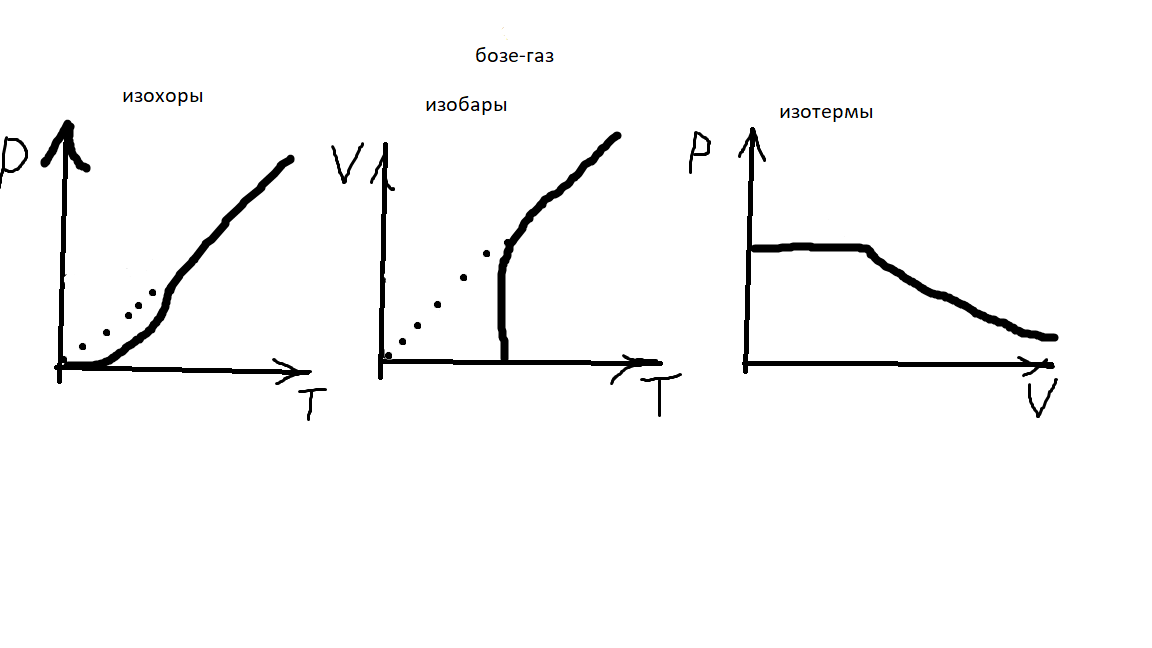
\includegraphics[width=0.7\linewidth]{bosegraphs}
	\caption{}
	\label{fig:fermigraphs}
\end{figure}





\end{ttask}


\begin{ttask}\textbf{12.} 
	
Построить изохоры, изобары и изотермы для ферми-газа. 

При $ T<<\varepsilon_{r} \quad p \approx \gamma\left(\frac{N}{v}\right)^{5 / 3} $




\begin{figure}[H]
	\centering
	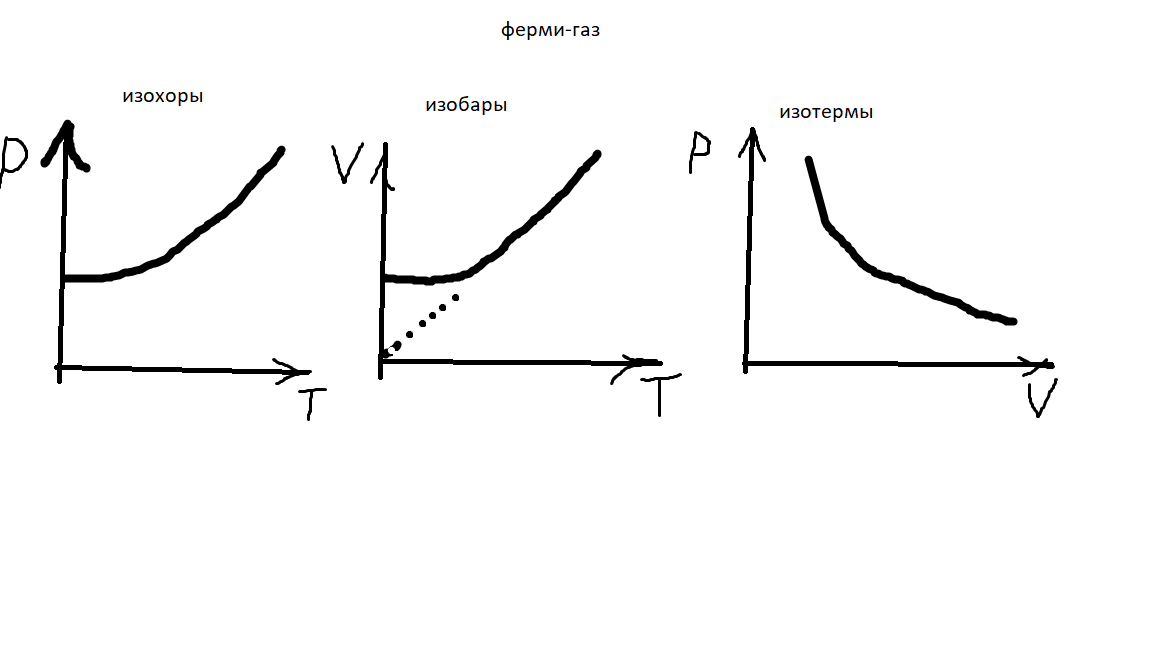
\includegraphics[width=0.7\linewidth]{fermi_graphs}
	\caption{}
	\label{fig:fermigraphs}
\end{figure}












\end{ttask}


\begin{ttask}\textbf{13.} 

Вычислить теплоемкость двумерного вырожденного идеального ферми-газа. 




\[ dN_p = g \bar{n}_p \frac{d p_x d p_y d V }{(2\pi \hbar)^2}=
\frac{g V p dp}{2\pi \hbar^2 \left(\exp \left(\frac{\varepsilon-\mu }{T}\right)+1 \right) }
 \]

\[\varepsilon=\frac{p^2}{2m} \Rightarrow  p dp=m d \varepsilon\]

\[ dN_\varepsilon= \left(\frac{g m }{2\pi \hbar^2}\right) V \frac{d \varepsilon }{e^{(\varepsilon-\mu)/T}+1}=
\left(\frac{g m }{2\pi \hbar^2}\right) V T \frac{dx}{e^{x-y}+1}
\]

\[ E= \left(\frac{g m }{2\pi \hbar^2}\right) V T^2 \int_{0}^{\infty}\frac{x dx}{e^{x-y}+1} \approx
\left(\frac{g m }{2\pi \hbar^2}\right) V T^2 \left(  \left(\frac{\mu^2}{2T^2}\right)+\frac{\pi^2}{6}\right)\]


\[ C=\frac{1}{V}\frac{dE}{dT}=
\left(  \frac{g m }{2\pi \hbar^2}\right)\frac{\pi^2}{3} T\]














\end{ttask}


\begin{ttask}\textbf{14}. 

Вычислить теплоемкость черного излучения. 



Химический потенциал
фотонного газа равен нулю. 

Распределение фотонов дается
соотношением:
\[ \bar{n}=\frac{1}{\operatorname{exp}\left(\frac{\hbar \omega_{k}}{T}\right)-1} \]

Число состояний определяется соотношением
$$
2 \frac{V 4 \pi k^{2} d k}{(2 \pi)^{3}}=2 \frac{V 4 \pi \omega_{k}^{2} d \omega_{k}}{(2 \pi c)^{3}}
$$

Дополнительный фактор 2 возникает из-за двух поляризаций фотонов.

Подставляя это число в $ \bar{N_{n}}$, получаем:
$$
d N_{\omega}=\frac{1}{\exp (\hbar \omega / T)-1} \frac{V \omega^{2} d \omega}{\pi^{2} c^{3}}
$$
Энергия излучения получается из $ d N_{\omega} $ умножением на энергию фотона
\begin{equation}\label{plank}
d E_{\omega}=
\frac{1}{\exp (\hbar \omega / T)-1} \frac{V \hbar \omega^{3} d \omega}{\pi^{2} c^{3}}
\end{equation}
Формула \ref{plank} - называется формулой Планка. 

Дальше считаем свободную энергию.
$$
	F=T \sum_{k} \ln \left[1-\exp \left(-\frac{\varepsilon_{k}}{T}\right)\right]
	=T \frac{V}{\pi^{2} c^{3}} \int_{0}^{\infty} \omega^{2} \ln \left[1-\exp \left(-\frac{\hbar \omega}{T}\right)\right] d \omega
$$
Заменяя переменную интегрирования $\quad x=\hbar \omega / T \quad$ и интегрируя по
частям, отсюда получим
$$
F=-\frac{V T^{4}}{3 \pi^{2} \hbar^{3} c^{3}} \int_{0}^{\infty} \frac{x^{2} d x}{\exp (x)-1}
$$
Безразмерный интеграл в этом соотношении равен $\pi^{4} / 15 .$ Итак, свободная энергия равна
$$
F=-\frac{\pi^{2} V T^{4}}{45 \hbar^{3} c^{3}}=-\frac{4 \sigma}{3 c} V T^{4}
$$


Коэффициент $\sigma$ называется постоянной Стефана-Больцмана:
$$
\sigma=\frac{\pi^{2} k^{4}}{60 \hbar^{3} c^{2}}=5.67 \cdot 10^{-5} \frac{\text{г}}{\text{сек}^{3}\text{град}^{4} }
$$
(если температура измеряется в градусах Кельвина). Зная свободную энергию, определяем обычную энергию (закон Больцмана)
$$
E=F-T\left(\frac{\partial F}{\partial T}\right)_{V}=\frac{4 \sigma}{c} V T^{4}
$$
Для теплоемкости излучения в полости с заданным объемом получаем
$$
C_{V}=\frac{16 \sigma}{c} V T^{3}
$$


















 

\end{ttask}


\begin{ttask}\textbf{15}

Найти равновесную плотность и теплоемкость акустических фононов в кристалле при температурах выше $ T $  и ниже $ T $  дебаевской




Гамильтониан атомов решётки кристалла может быть диагонализирован, 
т. е. разложен по нормальным модам колебаний. 
В представлении вторичного квантования он имеет вид



$$
	\hat{H}=\sum_{\mathbf{k}} \frac{1}{2}\left(\mathbf{p}_{\mathbf{k}}^{2}+\omega_{\mathbf{k}}^{2} \mathbf{q}_{\mathbf{k}}^{2}\right)=\sum_{\mathbf{k}, \text { З поляризац.}}  \hbar \omega_{\mathbf{k}}\left(\hat{a}_{\mathbf{k}}^{+} \hat{a}_{\mathbf{k}}+\frac{1}{2}\right)
$$
Где $\hat{a}_{\mathbf{k}}^{+}$ оператор рождения, $n_{\mathbf{k}}=\hat{a}_{\mathbf{k}}^{+} \hat{a}_{\mathbf{k}}-$ числа заполнения мод. 
Мы ограничимся рассмотрением только акустических мод колебаний $\omega_{\mathrm{k}}=v_{l, t} \cdot k,$ 
поскольку при низких температурах в системе возбуждаются состояния с минимальными частотами. 
У звука в кристалле есть две поперечные моды со скоростью звука $v_{t}$ и одна продольная со скоростью звука
$v_{l},$ так что плотность числа состояний
$$
g(\omega)=\frac{V \omega^{2} d \omega}{2 \pi^{2}}\left(\frac{1}{v_{l}^{3}}+\frac{2}{v_{t}^{3}}\right)
$$
которую для краткости мы будем записывать как
$$
g(\omega)=\frac{3}{2} \cdot \frac{\omega^{2} d \omega}{\pi^{2} v^{3}}
$$
введя эффективную скорость звука $v:$


$$
\frac{3}{v^{3}}=\frac{2}{v_{t}^{3}}+\frac{1}{v_{l}^{3}}
$$
Поскольку фононы являются возбуждениями не пустого пространства, а коллективными колебаниями «пустого» кристалла, 
состоящего из $N$ атомов, существует важное отличие их одночастичных состояний от фотонов. 
В $\mathbf{k}$ -пространстве фононные состояния занимают только конечную сферу Дебая с радиусом $k_{D}$. 
Действительно, число степеней свободы кристалла равно числу его атомов $3 N$, 
значит столько же «точек» одночастичных состояний должно быть в сфере Дебая:
$$
\frac{3 V}{2 \pi^{2} v^{3}} 
\cdot 
\int_{0}^{\omega_{D}} \omega^{2} d \omega
=3 N
$$
где частота Дебая есть
$$
\omega_{D}
=
c k_{D}
=
v\left(\frac{6 \pi^{2} N}{V}\right)^{1 / 3}
$$



Физический смысл этого ограничения ясен: длина волны фонона не может быть меньше 
постоянной решётки $a=(V / N)^{1 / 3},$ а его частота, соответ-
ственно, должна быть меньше дебаевской $\omega \leq 2 \pi v / a \sim \omega_{D} .$ 
Тогда энергия идеального газа фононов в этом приближении равна
$$
E(T)=\int_{0}^{\omega_{D}} \frac{3 V \omega^{2}}{2 \pi^{2} v^{3}} \cdot \frac{\hbar \omega}{e^{\frac{h \omega}{T}}-1} d \omega
=
\frac{3 V T^{4}}{2 \pi^{2} v^{3} \hbar^{3}} \cdot \int_{0}^{\Theta_{D} / T} \frac{x^{3} d x}{e^{x}-1}
$$
Энергия $E(T)$ существенно зависит от величины температуры Дебая:
$\Theta_{D}=\hbar \omega_{D} .$ 


При низких температурах $T \ll \Theta_{D}$ верхний предел интегрирования можно заменить на $\infty$, 
и фононный газ ведёт себя так же, как тепловое излучение. 
Для его теплоемкости получаем закон Дебая:
$$
C_{V}(T)=\frac{12 \pi^{4}}{5} N\left(\frac{T}{\Theta_{D}}\right)^{3} \propto T^{3}
$$




При высоких температурах $T \gg \Theta_{D}$ все состояния сферы Дебая заполнены, 
и мы получаем закон равнораспределения по степеням свободы Дюлонга-Пти:
$$
C_{V}=3 N
$$




\end{ttask}


\begin{ttask}\textbf{16}

Используя представление оператора смещения гармонического осциллятора 

$\hat{x}=\left(\frac{\hbar}{2 m \omega}\right)^{1 / 2}\left(\hat{b}^{+}+\hat{b}\right),$ 
получить формулу $\left\langle e^{i k \hat{x}}\right\rangle=$
$=e^{-\frac{k^{2} \hbar}{4 m \omega}}$ при температуре $T=0$











Вспомним упражнение 11:




$$
\langle\exp (i k \hat{x})\rangle=\left\langle\exp \left(i k \sqrt{\frac{\hbar}{2 m \omega}}\left(\hat{a}_{\vec{p}}^{\dagger}+\hat{a}_{\vec{p}}\right)\right)\right\rangle =
$$


а так как
$$
\left[\hat{a}_{\vec{p}}, \hat{a}_{\vec{p}}^{\dagger}\right]=1
$$

то



$$
=\left\langle\exp \left(i k \sqrt{\frac{\hbar}{2 m \omega}} \hat{a}_{\vec{p}}^{\dagger}\right) \exp \left(i k \sqrt{\frac{\hbar}{2 m \omega}} \hat{a}_{\vec{p}}\right) \exp \left(\frac{1}{2} k^{2} \frac{\hbar}{2 m \omega}\left[\hat{a}_{\vec{p}}^{\dagger}, \hat{a}_{\vec{p}}\right]\right)\right\rangle=
$$

дальше экспоненты запишем через суммы и воспользуемся
$\left\langle\left(\hat{a}_{\vec{p}}^{\dagger}\right)^{n}\left(\hat{a}_{\vec{p}}\right)^{m}\right\rangle
=
\delta_{m n}
\left\langle\left(\hat{a}_{\vec{p}}^{\dagger}\right)^{n}\left(\hat{a}_{\vec{p}}\right)^{n}\right\rangle$


имеем:



$$
=\left\langle\sum_{n=0}^{+\infty}\left(\frac{1}{(n) !}\left(i k \sqrt{\frac{\hbar}{2 m \omega}} \hat{a}_{\vec{p}}^{\dagger}\right)^{n}\right) \sum_{m=0}^{+\infty}\left(\frac{1}{(m) !}\left(i k \sqrt{\frac{\hbar}{2 m \omega}} \hat{a}_{\vec{p}}\right)^{m}\right) \exp \left(-\frac{1}{2} \frac{k^{2} \hbar}{2 m \omega}\right)\right\rangle=
$$


$$
=\sum_{n=0}^{+\infty}\left(\left(\frac{1}{n !}\right)^{2}\left(-k^{2} \frac{\hbar}{2 m \omega}\right)^{n}\left\langle\left(\hat{a}_{\vec{p}}^{\dagger}\right)^{n}\left(\hat{a}_{\vec{p}}\right)^{n}\right\rangle\right) 
\exp \left(-\frac{1}{2} \frac{k^{2} \hbar}{2 m \omega}\right)
$$


Что ж, нужно посчитать среднее:


$$
\left\langle\left(\hat{a}_{\vec{p}}^{\dagger}\right)^{n}\left(\hat{a}_{\vec{p}}\right)^{n}\right\rangle=\frac{\operatorname{tr}\left(\exp (-\tau \hat{H})\left(\hat{a}_{\vec{p}}^{\dagger}\right)^{n}\left(\hat{a}_{\vec{p}}\right)^{n}\right)}{\operatorname{tr}(\exp (-\tau \hat{H}))}
$$

$$
\frac{t r\left(\exp (-\tau \hat{H})\left(\hat{a}_{\vec{p}}^{\dagger}\right)^{n}\left(\hat{a}_{\vec{p}}\right)^{n-1} \hat{a}_{\vec{p}}\right)}{t r(\exp (-\tau \hat{H}))}
$$




$$
\frac{t r\left(\exp (-\tau \hat{H})\left(\hat{a}_{\vec{p}}^{\dagger}\right)^{n}\left(\hat{a}_{\vec{p}}\right)^{n-1} \exp (-\tau \hat{H}) \exp (\tau \hat{H}) \hat{a}_{\vec{p}} \exp (-\tau \hat{H}) \exp (\tau \hat{H})\right)}{t r(\exp (-\tau \hat{H}))}
$$



$$
\frac{\operatorname{tr}\left(\exp (-\tau \hat{H})\left(\hat{a}_{\vec{p}}^{\dagger}\right)^{n}\left(\hat{a}_{\vec{p}}\right)^{n-1} \exp (-\tau \hat{H}) \hat{a}_{\vec{p}}^{(M)}(\tau) \exp (\tau \hat{H})\right)}{\operatorname{tr}(\exp (-\tau \hat{H}))}=
$$




$$
=\frac{\operatorname{tr}\left(\exp (-\tau \hat{H})\left(\hat{a}_{\vec{p}}^{\dagger}\right)^{n}\left(\hat{a}_{\vec{p}}\right)^{n-1} \exp (-\tau \hat{H}) \exp (-\epsilon \tau) \hat{a}_{\vec{p}} \exp (\tau \hat{H})\right)}{\operatorname{tr}(\exp (-\tau \hat{H}))}
$$




$$
\frac{\operatorname{tr}\left(\left(\hat{a}_{\vec{p}}^{\dagger}\right)^{n}\left(\hat{a}_{\vec{p}}\right)^{n-1} \exp (-\tau \hat{H}) \hat{a}_{\vec{p}}\right)}{t r(\exp (-\tau \hat{H}))} \exp (-\epsilon \tau)=
$$


$$
=\frac{\operatorname{tr}\left(\exp (-\tau \hat{H}) \hat{a}_{\vec{p}}\left(\hat{a}_{\vec{p}}^{\dagger}\right)^{n}\left(\hat{a}_{\vec{p}}\right)^{n-1}\right)}{\operatorname{tr}(\exp (-\tau \hat{H}))} \exp (-\epsilon \tau)=
$$


$$
=\left\langle\hat{a}_{\vec{p}}\left(\hat{a}_{\vec{p}}^{\dagger}\right)^{n}\left(\hat{a}_{\vec{p}}\right)^{n-1}\right\rangle \exp (-\epsilon \tau)=
$$



и так как


$$
\left[\hat{a}_{\vec{p}},\left(\hat{a}_{\vec{p}}^{\dagger}\right)^{n}\right]=n\left(\hat{a}_{\vec{p}}^{\dagger}\right)^{n-1}
$$


то


$$
=\left\langle\left(\left(\hat{a}_{\vec{p}}^{\dagger}\right)^{n} \hat{a}_{\vec{p}}+n\left(\hat{a}_{\vec{p}}^{\dagger}\right)^{n-1}\right)\left(\hat{a}_{\vec{p}}\right)^{n-1}\right\rangle \exp (-\epsilon \tau)
$$


$$
\left(\left\langle\left(\hat{a}_{\vec{p}}^{\dagger}\right)^{n}\left(\hat{a}_{\vec{p}}\right)^{n}\right\rangle+n\left\langle\left(\hat{a}_{\vec{p}}^{\dagger}\right)^{n-1}\left(\hat{a}_{\vec{p}}\right)^{n-1}\right\rangle\right) \exp (-\epsilon \tau)
$$



В итоге



$$
\left\langle\left(\hat{a}_{\vec{p}}^{\dagger}\right)^{n}\left(\hat{a}_{\vec{p}}\right)^{n}\right\rangle=\frac{n}{1-\exp (-\epsilon \tau)} \exp (-\epsilon \tau)\left\langle\left(\hat{a}_{\vec{p}}^{\dagger}\right)^{n-1}\left(\hat{a}_{\vec{p}}\right)^{n-1}\right\rangle=
$$



$$
=\frac{n \cdot(n-1) \cdot \ldots \cdot 2}{(1-\exp (-\epsilon \tau))^{n-1}} \exp (-(n-1) \epsilon \tau)\left\langle\hat{a}_{\vec{p}}^{\dagger} \hat{a}_{\vec{p}}\right\rangle=
$$


$$
\frac{(n) !}{(1-\exp (-\epsilon \tau))^{n-1}} \exp (-(n-1) \epsilon \tau) \frac{1}{\exp (\epsilon \tau)-1}
$$


$$
=\frac{(n) !}{(1-\exp (-\epsilon \tau))^{n-1}} \exp (-(n-1) \epsilon \tau) \frac{\exp (-\epsilon \tau)}{1-\exp (-\epsilon \tau)}=
$$


$$
=\frac{(n) !}{(1-\exp (-\epsilon \tau))^{n}} \exp (-n \epsilon \tau)
$$

Теперь осталось подставить.






$$
\langle\exp (i k \hat{x})\rangle=
$$


$$
=\sum_{n=0}^{+\infty}\left(\frac{1}{(n) !}\left(-k^{2} \frac{\hbar}{2 m \omega}\right)^{n} \frac{\exp (-n \epsilon \tau)}{(1-\exp (-\epsilon \tau))^{n}}\right) \exp \left(-\frac{1}{2} \frac{k^{2} \hbar}{2 m \omega}\right)
$$


$$
=
\\sum_{n=0}^{+\infty}\left(\frac{1}{(n) !}\left(-k^{2} \frac{\hbar}{2 m \omega}\right)^{n}\left(\frac{\exp (-\hbar \omega \tau)}{1-\exp (-\hbar \omega \tau)}\right)^{n}\right) \exp \left(-\frac{1}{2} \frac{k^{2} \hbar}{2 m \omega}\right)
$$


$$
=\exp \left(-\frac{k^{2} \hbar}{2 m \omega}\left(\frac{\exp (-\hbar \omega \tau)}{1-\exp (-\hbar \omega \tau)}+\frac{1}{2}\right)\right)
$$



$$
=\exp \left(-\frac{k^{2} \hbar}{4 m \omega} \frac{1+\exp (-\hbar \omega \tau)}{1-\exp (-\hbar \omega \tau)}\right)
$$



$$
=\exp \left(-\frac{k^{2} \hbar}{4 m \omega} \operatorname{coth}\left(\frac{\hbar \omega \tau}{2}\right)\right)
$$




Ответ:



$$
\langle\exp (i k \hat{x})\rangle=\exp \left(-\frac{k^{2} \hbar}{4 m \omega} \operatorname{coth}\left(\frac{\hbar \omega \tau}{2}\right)\right)
$$





решение задачи получается, если 
доказать, что для бозевских операторов рождения и уничтожения $\hat{b}_{i}^{+}, \hat{b}_{i}$ имеет место тождество
$$
e^{\tau\left(\hat{b}^{+}+\hat{b}\right)}=e^{\tau \hat{b}^{+}} e^{\tau \hat{b}} \exp \left(\tau^{2} / 2\right)
$$


Обозначим 
$ \hat{S}=e^{-\tau \hat{b}^{+}} e^{\tau\left(\hat{b}^{+}+\hat{b}\right)} $ 
и теперь

\[ \begin{array}{l}
	\frac{d \hat{S}}{d \tau}=e^{-\tau b^{+}}\left(-\hat{b}^{+}+\left(\hat{b}^{+}+\hat{b}\right)\right) e^{\tau\left(\hat{b}^{+}+\hat{b}\right)}=\left(e^{-\tau \hat{b}^{+}} \hat{b} e^{\tau \hat{b}^{+}}\right) e^{-\tau \hat{b}^{+}} e^{\tau\left(\hat{b}^{+}+\hat{b}\right)}= \\
	=\hat{b}(\tau) \hat{S}, \frac{d \hat{b}(\tau)}{d \tau}=e^{-\tau \hat{b}^{+}}\left(-\hat{b}^{+} \hat{b}+\hat{b} \hat{b}^{+}\right) e^{\tau \hat{b}^{+}}=1, \hat{b}(\tau)=\tau+\hat{b}
\end{array} \]


\[ \begin{array}{l}
	\text { поэтому } \frac{d \hat{S}}{d \tau}=(\tau+\hat{b}) \hat{S}, \hat{S}=\exp \left(\tau^{2} / 2\right), \tau^{\tau}, \text { следовательно, } \\
	e^{\tau\left(\dot{b}^{+}+\hat{b}\right)}=e^{-\hat{b}^{+}} e^{t \hat{b}} \exp \left(\tau^{2} / 2\right)
\end{array} \]






Теперь формула из условий очевидно, просто выносятся бозеевские операторы, а в экспоненте оказывается то, что нужно.















\end{ttask}




\begin{ttask} \textbf{17}


Описать парамагнетизм Паули и диамагнетизм Ландау. 
Рассмотреть эффект де Гааза–ван Альфена в двумерном металле. 




Парамагнетизм.


Наиболее просто намагниченность вычисляется в высокотемпературном пределе $T \gg T_{\text {выр}}$. 
В высокотемпературном приближении электронный газ больцмановский, 
его статистическая сумма факторизуется и достаточно вычислить её для одной частицы в поле $\mathcal{B}.$ 

Парамагнетизм связан с наличием у электрона собственного магнитного момента $\mu_{B}=e \hbar / 2 m c,$ 
так что его энергия в поле есть $\pm \mu_{B} \mathcal{B} .$ 
Вводя для удобства $x=\mu_{B} \mathcal{B} / T,$ получаем в расчете на один электрон
$$
\begin{array}{c}
	z=e^{-\frac{\mu_{B} B}{T}}+e^{\frac{\mu_{B} B}{T}}=2 \operatorname{ch} x 
	\\
	f=-T \ln z
	=
	-T \ln (2 \operatorname{ch} x) 
	\\
	m=-\left(\frac{\partial f}{\partial \mathcal{B}}\right)
	=
	\mu_{B} \frac{\partial}{\partial x} \ln (2 \operatorname{ch} x)
	=
	\mu_{B} \operatorname{th} x
\end{array}
$$
Полученная формула  имеет ясный физический смысл. 
В нулевом поле температура «размешивает» моменты электронов по направлениям, 
и магнитный момент газа отсутствует. 
При небольших полях $\mu_{B} \mathcal{B} \ll T$ наведённый магнитный момент линеен по полю, и удобно ввести


Восприимчивость $\chi$ в расчете на одну частицу определяется как 
$\chi=\lim _{\mathcal{B} \rightarrow 0} m / \mathcal{B} .$ 

Поэтому получаем $\chi=\mu_{B}^{2} / T .$

Эта зависимость называется законом Кюри и показывает, что при больших температурах магнетизм исчезает.






Кроме положительной парамагнитной восприимчивости, существует еще 
отрицательная диамагнитная восприимчивость. 

Диамагнетизм возникает из-за дискретности уровней Ландау энергии электронов $\varepsilon_{n}=\hbar \omega(n+1 / 2)$
кратностью $\quad$ вырождения $ g_{L}=\mathcal{B} S / \Phi_{0}$. 

Здесь $\hbar \omega=2 \mu_{B} \mathcal{B}-$ циклотронная частота, 
а $\Phi_{0}=2 \pi \hbar c / e-$ квант потока, так
что кратность вырождения уровня Ландау $g_{L}$ - это просто число квантов
потока $\Phi / \Phi_{0}$, проходящего через поперечное к полю сечение образца. В
этом случае одночастичная статсумма равна
$$
z
=
g_{L} \sum_{n=0}^{\infty} 
e^{-\frac{h \omega}{T}\left(n+\frac{1}{2}\right)}
=
\frac{g_{L}}{2 \operatorname{sh} x}
$$
где учтено, что $x=\hbar \omega / 2 T=\mu_{B}$ В $/ T$. Отсюда в расчете на один электрон
получаем
$$
\begin{array}{c}
	f=-T \ln z=-T \ln \frac{x}{\operatorname{sh} x}+\ldots 
	\\
	m=-\left(\frac{\partial f}{\partial \mathcal{B}}\right)
	=
	\mu_{B} \frac{\partial}{\partial x} \ln \frac{x}{\operatorname{sh} x}
	=
	-\mu_{B}\left(\operatorname{cth} x-\frac{1}{x}\right)
\end{array}
$$


Намагниченность описывается функцией Ланжевена: $m=-\mu_{B} \mathcal{L}(x),$ 
а диамагнитная восприимчивость
$$
\chi_{\text {диа }}=\left(\frac{\partial m}{\partial \mathcal{B}}\right)_{B=0}=-\frac{\mu_{B}^{2}}{3 T}
$$
в три раза меньше парамагнитной $\chi_{\text {диа}}=-\chi_{\text {пара}} / 3 .$ Таким образом, в целом
электронный газ парамагнитен: $\chi_{\text {диа}}+\chi_{\text {пара}}>0 .$



Если зеемановская энергия электронов становится больше температуры $T<\mu_{B} \mathcal{B} \ll \varepsilon_{F},$ то магнитное поле называют «квантующим». 
В этих условиях становится существенной дискретность уровней Ландау, что приводит к 
появлению у намагниченности электронного газа осциллирующей части. 
Амплитуда этих осцилляций не мала, а «шаг» осцилляций по обратному магнитному полю постоянен. 
Это доставляет ценную информацию о свойствах ферми-поверхности металла. Поэтому эффект заслужил имя собственное, де Гааза-ван Альфрена (1930). 
Для того, чтобы оценить амплитуду и «шаг» по полю осцилляций де Гааза-ван Альфена, 
рассмотрим самый простой случай: двумерный ( $\mathrm{D}=2$ ) электронный газ при нулевой температуре $(T=0) .$ Тогда в 
магнитном поле $N$ электронов газа распределены по уровням Ландау следующим образом. 
На уровнях $0,1,2, \ldots, j$ «сидит» по $g_{L}$ электронов, а на последнем $j+1$ -м уровне - оставшиеся $N-g_{L}(j+1)$ штук. 
Таким будет распределение электронов в интервале значений приложенного поля:
$$
\frac{(j+1)}{B_{0}}<\frac{1}{B}<\frac{(j+2)}{B_{0}}
$$
где $\mathcal{B}_{0}=N \Phi_{0} / 2 S, S-$ площадь образца, $g_{L}=2 B S / \Phi_{0}-$ кратность вырождения уровня Ландау с учетом спина. 


Вычислим энергию основного состояния газа при $T=0$ :
$$
\begin{array}{l}
	E=g_{L} \sum_{k=0}^{j} 
	\hbar \omega
	\left(k+\frac{1}{2}\right)
	+
	\hbar \omega
	\left(j+\frac{3}{2}\right)
	\left(N-g_{L}(j+1)\right)
	= \\
	=
	2 N \mu_{B}
	\left[
	\frac{B}{B_{0}}\left(j+\frac{3}{2}\right)
	-
	\left(\frac{\mathcal{B}}{B_{0}}\right)^{2}(j+1)\left(\frac{j}{2}+1\right)
	\right]
\end{array}
$$
При нулевой температуре свободная энергия совпадает с внутренней $F=E-T S$. 
Магнитный момент $M=-\partial E / \partial \mathcal{B}$ основного состояния 
электронного газа при нулевой температуре в указанном интервале полей равен
$$
M(\mathcal{B})
=
N \cdot \frac{e \hbar}{m c} \cdot
\left[
(j+1)(j+2) \frac{\mathcal{B}}{\mathcal{B}_{0}}
-
j-\frac{3}{2}
\right]
$$



При изменении магнитного поля последний уровень Ландау постепенно заполняется, пока число $j$ скачком не увеличится на единицу. В следующем
по $j \rightarrow j+1$ интервале обратных полей повторяется точно такая же зависимость $M(\mathcal{B})$. 
Таким образом, магнитный момент $M$ осциллирует в интервале $\pm N \mu_{B}$ с постоянным по обратному полю шагом:
$$
\frac{1}{\mathcal{B}_{0}}=\frac{e S}{\pi \hbar c N}=\frac{\mu_{B}}{\varepsilon_{F}}
$$
Физический смысл осцилляций намагниченности связан с периодическим заполнением и 
опорожнением последнего по счёту заполняемого уровня Ландау. 
Чтобы эти осцилляции были выражены и не «размывались» температурными эффектами, необходимо, 
чтобы поле было квантующим $T \ll \mu_{B} \mathcal{B},$ а 
электронный газ вырожденным $\mu_{B} \mathcal{B} \ll \varepsilon_{F} .$ 






























\end{ttask}


\begin{ttask}\textbf{18. }

Сравнить низкотемпературные зависимости теплоемкости идеальных бозе- и ферми-газов, 
черного излучения и твердого тела, 
парамагнетика и ферромагнетика, 
неидеального бозе-газа и, наконец, сверхпроводника. 



Вырожденные ферми- и бозе-газы $\left(T \ll T_{\text {выр}}\right)$ ведут себя очень по-
разному. 

Рассмотрим сначала ферми-газ. 

Запишем, как и ранее, выражение для энергии:
$$
E=B V \cdot \int_{0}^{\infty} 
\frac{\sqrt{\varepsilon} \cdot \varepsilon d \varepsilon}{e^{\frac{\varepsilon-\mu}{T}}+1}
$$
Низкотемпературные свойства фермионов определяются тем, 
что при $T=0$ сфера Ферми заполнена, а при увеличении температуры заполненность состояний изменяется 
в узком слое шириной $\sim T$ около поверхности Ферми. 
Как отмечалось выше, при $T \ll T_{\text {выр}}$ функция распределения Ферми-Дирака 
имеет вид резко выраженной «ступеньки», так что, полагая в $\mu=\mu(0),$ получаем
$$
E=
\frac{2}{5} B V \mu^{5 / 2}(0)
=
\frac{3}{2}PV
$$


Чтобы вычислить теплоёмкость вырожденного ферми-газа, 
нужно «выделить» отличие функции распределения Ферми-Дирака от «ступеньки». 
Это отличие мало в меру малости $T / \varepsilon_{F} \ll 1,$ то есть наш интеграл нужно разложить по этому малому параметру:

$$
\int_{0}^{\infty} \frac{f(\varepsilon) d \varepsilon}{e^{\frac{\varepsilon-\mu}{T}}+1}=\int_{0}^{\mu} f(\varepsilon) d \varepsilon+\frac{\pi^{2}}{6} T^{2} f^{\prime}(\mu)+\ldots
$$

Тогда
$$
E=\frac{2}{5} B V \mu^{5 / 2}
\left[
1
+
\frac{5 \pi^{2}}{8}\left(\frac{T}{\mu}\right)^{2}
+
\ldots
\right]
$$


Тогда


\[ C_{V}(T)=\frac{\pi^{2}}{2} \cdot N \cdot \frac{T}{\varepsilon_{F}}+\ldots \]



Здесь учтено, что  $2 B V \mu^{5 / 2}(0) / 5=3 N \varepsilon_{F} / 5$. 

Линейная зависимость теплоемкости от температуры имеет ясный физический смысл. 
При нулевой температуре сфера Ферми полностью заполнена. 
При нагревании газа до небольшой температуры $T$ происходит изменение чисел электронов только в узком слое $\sim T$ вблизи поверхности Ферми. 
Относительная доля электронов, переместившихся в возбужденные состояния, $\sim T / \varepsilon_{F}$, а изменение энергии каждого $\sim T$, 
так что теплоёмкость газа получается $C_{V} \sim N T / \varepsilon_{F}$.






Теперь вычислим теплоемкость бозе-газа, для этого найдем энергию. 
Поскольку $\varepsilon_{0}=0$ при $\mathbf{p}=0$ и $T<T_{B}$ получаем
$$
E=B V T^{5 / 2} \cdot \int_{0}^{\infty} \frac{x^{3 / 2} d x}{e^{x}-1}
$$
Здесь безразмерный интеграл в численно равен 1.78 , так что
$$
E \approx 0.77 \cdot N T\left(\frac{T}{T_{B}}\right)^{5 / 2}
$$
а теплоёмкость равна
$$
C_{V}
=
\frac{\partial E}{\partial T} 
\approx 
1.92 \cdot N\left(\frac{T}{T_{B}}\right)^{3 / 2} 
\propto 
T^{3 / 2}
$$




А для черного тела теплоемкость была найдена в задаче 14:
$$
C_{V}=\frac{16 \sigma}{c} V T^{3}
$$





Для теплоемкости твердого тела известен закон Дебая:
$$
C_{V}(T)=\frac{12 \pi^{4}}{5} N\left(\frac{T}{\Theta_{D}}\right)^{3} \propto T^{3}
$$



Для сверхпроводника по лекциям было получено выражение:

Тогда теплоемкость
$$
C_{s}
=
C_{n}+\frac{T_{c}}{2 A} \nu(0)
$$
то есть всё линейно, только при переходе в сверхпроводящее состояние имеется скачок.




теплоемкости диа и пара магнетиков определяются свойствами твердого тела и вкладом электронов, 
а это было уже описано выше.











\end{ttask}






\begin{ttask} \textbf{19.}
	 
Показать, что фазовая скорость элементарного возбуждения в бозе-конденсате равна гидродинамической скорости звука.



Рассмотрим бозе-конденсат.





рассмотрим неидеальный бозе-газ в ловушке $V(\vec{r})$, которая создается внешним магнитным полем. 

Для простоты ограничимся температурой, близкой к нулю, 
когда тепловых возбуждений очень мало 
$T \ll T_{c} \simeq\left(\hbar^{2} / m\right) n^{2 / 3}$. 

Полный гамильтониан системы имеет вид
$$
\hat{H}_{t o t}
=
\int d^{3} r\left[
\hat{\Psi}^{+}(t, \vec{r})
\left(\frac{\hat{p}^{2}}{2 m}+V(\vec{r})-\mu_{0}\right) 
\hat{\Psi}(t, \vec{r})
+
\frac{1}{2} U_{0} 
\hat{\Psi}^{+}(t, \vec{r}) \hat{\Psi}^{+}(t, \vec{r}) 
\hat{\Psi}(t, \vec{r}) \hat{\Psi}(t, \vec{r})
\right]
$$


Величина постоянной $\mu_{0}$ произвольна и, фактически, фиксирует начало отсчета энергии. 

Ниже ее значение будет выбрано так, чтобы функция основного состояния не зависела от времени. 

Имея ввиду описание явлений, слабо меняющихся на масштабах парного взаимодействия атомов, 
потенциальная энергия взаимодействия записана в локальной форме. 


Параметр $U_{0}$ имеет размерность энергия $\times$ объем и записывается в виде
$$
U_{0}=\frac{4 \pi \hbar^{2} a}{m}
$$
Величина $a$ называется длиной рассеяния. 



Производная по времени от гайзенберговских операторов равна
$$
i \hbar \frac{\partial}{\partial t} \hat{\Psi}(t, \vec{r})=[\hat{\Psi}(t, \vec{r}), \hat{H}]
$$
Приходим к нелинейному "уравнению Шредингера"
$$
i \hbar \frac{\partial}{\partial t} 
\hat{\Psi}(t, \vec{r})
=
\left(\frac{\hat{p}^{2}}{2 m}+V(\vec{r})-\mu_{0}\right) 
\hat{\Psi}(t, \vec{r})
+
U_{0} 
\hat{\Psi}^{+}(t, \vec{r}) 
\hat{\Psi}(t, \vec{r}) \hat{\Psi}(t, \vec{r})
$$



Разложим функцию бозе-поля $\hat{\Psi}$ 
по собственным функциям одночастичной задачи


\[ 
\begin{array}{c}
	\left(\frac{\hat{p}^{2}}{2 m}+V(\vec{r})-\mu_{0}\right) \varphi_{k}(\vec{r})=\xi_{k} \varphi_{k}(\vec{r}) \\
	\hat{\Psi}=\sum_{k} \hat{a}_{k}(t) \varphi_{k}(\vec{r})
\end{array} 
\]



Рассмотрим газ в отсутствии потенциала ловушки, 
когда функции $\varphi_{k}(\vec{r})=V^{-1 / 2} \exp (i \vec{k} \vec{r})$ 
суть плоские волны в ящике $V=L^{3}$ с периодическими граничными условиями 
$\varphi_{k}(\vec{r})=\varphi_{k}(\vec{r}+\vec{L})$. 



В основном состоянии (при нулевой температуре) все частицы идеального бозе-газа находятся в конденсате, 
т.е. имеют нулевой импульс. 

В неидеальном газе при $T=0$ большинство частиц $N_{0}$ остаются в конденсате, 
но из-за отталкивания небольшая доля частиц имеют ненулевые импульсы. 
Поэтому выделим оператор с нулевым импульсом: 
$\left\langle\hat{\Psi}_{1}\right\rangle=0 $
$$
\begin{aligned}
	\hat{\Psi} &=\varphi_{0}(\vec{r}) \hat{a}_{0}+\hat{\Psi}_{1},
	\\
	\hat{\Psi}_{1} &=\sum_{k \neq 0} \hat{a}_{k}(t) \varphi_{k}(\vec{r})
\end{aligned}
$$



Все наблюдаемые величины при низких температурах являются средними по состоянию конденсата. 

Поэтому, $ \hat{\Psi} $ первый член заменить на классическую функцию конденсата
$$
\hat{\Psi}=\Psi+\hat{\Psi}_{1}
$$



Амплитуда плотности конденсата $\Psi$ в слабо неравновесном случае есть классическое бозе-поле $\Psi(t, \vec{r})$,
аналогичное скалярному потенциалу классического электрического поля. 


Чтобы найти эволюцию конденсата, следует подставить
$\Psi(t, \vec{r})$ в уравнение его динамики 
и пренебречь операторной частью поля, 
описывающей надконденсатные частицы $\hat{\Psi}_{1}$. 
Имеем
$$
i \hbar \frac{\partial}{\partial t} \Psi(t, \vec{r})=\frac{\hat{p}^{2}}{2 m} \Psi(t, \vec{r})+U_{0} \Psi^{*}(t, \vec{r}) \Psi(t, \vec{r}) \Psi(t, \vec{r})-\mu_{0} \Psi(t, \vec{r})
$$


В физике сверхтекучего бозе-газа это уравнение называется уравнением Гросса-Питаевского (1961), 
которые первые обосновали возможность описания движения конденсата уравнением. 



Основное состояние этого уравнения однородно и не зависит от времени
$$
\Psi(t, \vec{r})=\Psi
$$
если введенная выше константа равна
$$
\mu_{0}=U_{0} \Psi^{2}
$$



Число частиц и энергия однородного конденсата связаны с амплитудой конденсата $\Psi$ формулами
$$
N_{0}
=
\int d^{3} r \Psi^{+} \Psi
=
\Psi^{2} V, 
\quad
E_{00}
=
\frac{1}{2} U_{0} \int d^{3} r \Psi^{+} \Psi^{+} \Psi \Psi
=
\frac{U_{0} N_{0}^{2}}{2 V}
$$


Дифференцируя энергию по числу частиц, находим химический потенциал
$$
\mu
=
\frac{\partial E_{00}}{\partial N_{0}}
=
\frac{U_{0} N_{0}}{V}
=
U_{0} \Psi^{2}
$$


Видим, что введенная ранее постоянная $\mu_{0}$ есть химический потенциал. 

При этом $E_{00}=\frac{1}{2} \mu_{0} N_{0} .$ 

В отличие от идеального газа, 
неидеальный бозе-газ в основном состоянии обладает отличным от нуля давлением
$$
P=-\frac{\partial E_{00}}{\partial V}=\frac{U_{0} N_{0}^{2}}{2 V^{2}}
$$
и гидродинамической скоростью звука




$$
c=\sqrt{\frac{\partial P}{\partial \rho}}=\sqrt{\frac{U_{0} \rho}{m^{2}}}=\sqrt{\frac{\mu_{0}}{m}}
$$
$\left(\rho=m N_{0} / V\right.$ - плотность газа ). Здесь мы пренебрегаем отличием $N_{0}$ от полного числа частиц $N$.




Таким образом, мы получили скорость звука.









Теперь рассмотрим элементарные возбуждения неидельного бозе-газа.


Даже при нулевой температуре небольшая часть частиц не принадлежит 
конденсату и имеет отличные от нуля импульсы. 
Свойства этих частиц описываются операторной функцией $\hat{\Psi}_{1}$. 

Эволюция этого оператора описывается линейной по $\hat{\Psi}_{1}$ 
частью основного уравнения 

\[ i \hbar \frac{\partial}{\partial t} \hat{\Psi}(t, \vec{r})
=
\left(\frac{\hat{p}^{2}}{2 m}+V(\vec{r})-\mu_{0}\right) 
\hat{\Psi}(t, \vec{r})
+
U_{0} \hat{\Psi}^{+}(t, \vec{r}) \hat{\Psi}(t, \vec{r}) \hat{\Psi}(t, \vec{r}) \]


то есть решаем уравнение:
$$
i \hbar \frac{\partial}{\partial t} \hat{\Psi}_{1}(t, \vec{r})
=
\frac{\hat{p}^{2}}{2 m} \hat{\Psi}_{1}(t, \vec{r})
+
2 U_{0} \Psi^{2} \hat{\Psi}_{1}(t, \vec{r})
+
U_{0} \Psi^{2} \hat{\Psi}_{1}^{+}(t, \vec{r})
-
\mu \hat{\Psi}_{1}(t, \vec{r})
$$




С учетом $\mu_{0}=U_{0} \Psi^{2}$ приводим это уравнение к компактному виду
$$
i \hbar \frac{\partial}{\partial t} \hat{\Psi}_{1}
=
\left(\frac{\hat{p}^{2}}{2 m}+\mu\right) \hat{\Psi}_{1}+\mu \hat{\Psi}_{1}^{+}
$$

Подставим разложение по собственным функциям одночастичной задачи:
$$
i \hbar \frac{\partial}{\partial t} \hat{a}_{k}(t)=\xi_{k} \hat{a}_{k}(t)+\mu \hat{a}_{-k}^{+}(t)
$$


В этом уравнении удивительным образом перемешаны бозе-операторы $\hat{a}_{k}(t)$ и $\hat{a}_{-k}^{+}(t) .$ 

Первый член справа описывает свободное движение частицы, 
а последний член в приближении самосогласованного поля 
отражает виртуальное поглощение частицы конденсатом.





далее преобразование Боголюбова



Для диагонализации последнего уравнения  применим каноническое преобразование Боголюбова:
$$
\hat{a}_{k}(t)=\left[u_{k} \hat{b}_{k} e^{-i \varepsilon_{k} t / \hbar}-v_{k} \hat{b}_{-k}^{+} e^{i \varepsilon_{k} t / \hbar}\right]
$$
и его эрмитово сопряженное выражение (с заменой знака импульса)
$$
\hat{a}_{-k}^{+}(t)=\left[u_{k} \hat{b}_{-k}^{+} e^{+i \varepsilon_{k} t / \hbar}-v_{k} \hat{b}_{k} e^{-i \varepsilon_{k} t / \hbar}\right]
$$
Здесь введены операторы поглошения $\hat{b}_{k}$ и рожления $\hat{b}_{k}^{+}$ квазичастиІ, которые удовлетворяют таким же правилам коммутаІии, что и исходные операторы "голых частиІ".



$$
\left[\hat{b}_{k}, \hat{b}_{k^{\prime}}^{+}\right]=\delta_{k, k^{\prime}}, \quad\left[\hat{b}_{k}, \hat{b}_{k^{\prime}}\right]=\left[\hat{b}_{k}^{+}, \hat{b}_{k^{\prime}}^{+}\right]=0
$$
Отсюда
$$
u_{k}^{2}-v_{k}^{2}=1
$$



В рассматриваемом приближении квазичастицы ведут себя как частиІы идеального газа, и соответсвуюшие операторы являются собственными "функциями" оператора энергии
$$
i \hbar \frac{\partial}{\partial t} \hat{b}_{k}=\varepsilon_{k} \hat{b}_{k}, i \hbar \frac{\partial}{\partial t} \hat{b}_{k}^{+}=-\varepsilon_{k} \hat{b}_{k}^{+}
$$
с неизвестными пока собственными значениями $\pm \varepsilon_{k} .$ КоэффиІиенты преобразования $u_{k}, v_{k}$ полагаются действительными, четными функциями вектора $k .$ Это всегда можно сделать удачным выбором фаз у операторов $\hat{b}_{k}$.



Смысл формулы (126) состоит в том, что поглощение бозе-частицы, из состояния с импульсом $k$ 
эквивалентно поглощению с вероятностью $u_{k}^{2}$ конденсатом одного кванта элементарного возбуждения и 
рождению с вероятностью $v_{k}^{2}$ из конденсата кванта с противоположным импульсом. 


Подставив преобразование Боголюбова, находим энергию квазичастицы
$$
\varepsilon_{k}=\sqrt{\xi_{k}^{2}-\mu^{2}}=\sqrt{\frac{(\hbar k)^{2}}{m} \mu+\left(\frac{(\hbar k)^{2}}{2 m}\right)^{2}}
$$



и коэффициенты преобразования
$$
u_{k}=\sqrt{\frac{1}{2}\left(\frac{\xi_{k}}{\varepsilon_{k}}+1\right)}, 
\quad
v_{k}=\sqrt{\frac{1}{2}\left(\frac{\xi_{k}}{\varepsilon_{k}}-1\right)}, 
\quad
u_{k}^{2}+v_{k}^{2}=\frac{\xi_{k}}{\varepsilon_{k}}, 
\quad
2 u_{k} v_{k}=\frac{\mu}{\varepsilon_{k}}
$$




Фактически, это коэффициенты поворота в пространстве 
с гиперболической метрикой $u_{k}^{2}-v_{k}^{2}=1$.






При больших импульсах $\varepsilon_{k}$ совпадает с энергией свободной частицы
$$
\varepsilon_{k} \simeq \frac{(\hbar k)^{2}}{2 m}, 
\quad 
\varepsilon_{k} \gg \mu
$$
а длинноволновая часть спектра имеет форму звукового спектра, т.е. линейно зависит от импульса.
$$
\varepsilon_{k}=c \hbar k, \quad c=\sqrt{\frac{\mu}{m}}=\sqrt{\frac{U_{0} N_{0}}{m V}}, \quad \varepsilon_{k} \ll \mu
$$
Величина $c$ численно равна гидродинамической скорости звука, которая найдена в первой половине задачи. 














\end{ttask}



\begin{ttask} \textbf{20}

Найти распределение частиц по импульсам и полное число надконденсатных частиц в идеальном и неидеальном бозе-газах при T = 0 и низких температурах.





В случае идеального бозе-газа число надкондексатных частиц известно:
\[ N_{0}=N\left[1-\left(\frac{T}{T_{c}}\right)^{3 / 2}\right] 
\]

Получим его:


Полное число частиц
$$
N=\sum_{p} N_{p}=\sum_{p} \frac{1}{e^{\beta\left(\varepsilon_{p}-\mu\right)}-1}
$$
не зависит от температуры и, тем самым неявным образом залает зависимость химического потенциала от температуры. 

Преобразуем его с помощью правила Бора-Зоммерфельда, согласно которому для любой функции 
от энергии сумма по импульсам эквивалентна интегралу
$$
I=
\sum_{p} f\left(\varepsilon_{p}\right)=
\int \frac{L^{3} d^{3} p}{(2 \pi \hbar)^{3}} f\left(\varepsilon_{p}\right)=
\nu V \int_{0}^{\infty} \varepsilon^{1 / 2} d \varepsilon f(\varepsilon)
$$
где $\nu=\frac{m^{3 / 2}}{2^{1 / 2} \pi^{2} \hbar^{3}} .$ 


Поэтому, переобозначив $z=p^{2} / 2 m T$, полное число частиц станет
$$
N=T^{3 / 2} \nu V \int_{0}^{\infty} \frac{z^{1 / 2} d z}{e^{z} e^{-\beta \mu}-1}.
$$


Исследуем это выражение для поиска $ \mu(T) $. 
Запишем его в виде:
$$
\int_{0}^{\infty} \frac{z^{1 / 2} d z}{e^{z} e^{-\beta \mu}-1}=\frac{N}{T^{3 / 2} \nu V}
$$
Чтобы при росте температуры интеграл падал как $T^{-3 / 2},$ необходимо падение подынтегрального выражения, 
т.е. член $e^{z-\beta \mu}$ должен расти с $z$.
Поэтому при достаточно высоких температурах единицей в 
подынтегральном выражении можно пренебречь и, считая $ \mu(T)\ne \mu(z)$, 
запишем равенство через гамма функцию:
%
$$
N=\Gamma(3 / 2) T^{3 / 2} \nu V e^{\beta \mu},
$$
поэтому $e^{\beta \mu} \sim T^{3 / 2}$ и видим понижение химического потенциала по закону
$$
\mu \sim-\frac{3}{2} T \ln \frac{1}{T}
$$

И видим, что при больших температурах в знаменателе распределения Бозе-Эйнштейна можно пренебречь единицей и перевести 
распределение Бозе в распределение Максвелла-Больцмана
$$
N_{p}=e^{\beta\left(\mu-\varepsilon_{p}\right)}
$$


А если дальше понижать температуру, то уже невозможно, чтобы выполнялось исследуемое уравнение, 
потому что уже стабильно $\mu=0 .$ 
А так как мы его получили из правила Бора-Зоммерфельда, то понятно, что нужно как-то иначе его применить.
Так как в области низких температур число частиц на нижнем уровне $N_{0}$ очень велико, 
то следует заменять сумму на интеграл только для возбужденных состояний плюс число частиц на нулевом уровне
$$
N=\sum_{p} N_{p}
=
N_{0}+T^{3 / 2} \nu V 
\int_{0}^{\infty} d z 
\frac{z^{1 / 2}}{e^{z}-1}
$$


В итоге выражаем находим температурную зависимость числа $N_{0}:$
$$
N_{0}=N\left[1-\left(\frac{T}{T_{c}}\right)^{3 / 2}\right]
$$





Рассмотрим неидеальный бозе-газ



Из преобразований Боголюбова следует, что среднее по состоянию газа число частиц с импульсом $k$ равно
$$
N_{k}=\left\langle\hat{a}_{k}^{+} \hat{a}_{k}\right\rangle=v_{k}^{2}+u_{k}^{2}\left\langle\hat{b}_{k}^{+} \hat{b}_{k}\right\rangle+v_{k}^{2}\left\langle\hat{b}_{-k}^{+} \hat{b}_{-k}\right\rangle
$$
При нулевой температуре квазичастицы отсутствуют, и первый член здесь дает
$$
N_{k}^{(0)}
=
v_{k}^{2}
=
\frac{1}{2}\left(
\frac{\xi_{k}}{\varepsilon_{k}}-1
\right)
$$
При $\varepsilon_{k} \ll \mu$ это число весьма велико, но при $\varepsilon_{k} \gg \mu$ быстро падает. 
Полное число надконденсатных частиц по порядку величины равно, очевидно, 
числу состояний свободных частиц с импульсами меньше $p_{\max }=\sqrt{2 m \mu} .$ 
Это число равно
$$
n_{1}^{(0)}
=
\frac{1}{V} \sum N_{k}^{(0)} 
\simeq 
\frac{p_{\max }^{3}}{(2 \pi \hbar)^{3}} 
\simeq 
n_{0} \sqrt{n_{0} a^{3}}
$$
Теория Боголюбова опирается на предположение, 
что в основном состоянии большинство частиц находится в конденсате, и $n_{1}^{(0)} \ll n_{0} .$ 


Отсюда находим оценку максимальной плотности газа
\[ \max n_{0} \simeq a^{-3} \]


В зависимости от рассматриваемой области температур плотность возбужденных частиц по порядку величины равна



$$
\begin{aligned}
	n_{1}^{(T)} & \simeq \frac{\mu}{T}\left(\frac{T}{c}\right)^{3}, 0<T<\mu \\
	n_{1}^{(T)} & \simeq \sum N_{k} \simeq(m T)^{3 / 2}, \mu<T \ll T_{c} \frac{\mu}{T_{c}}=a n^{1 / 3}
\end{aligned}
$$
Подчеркнем, что энтропия конденсата равна нулю, и при $T \ll T_{c}$ вклад в энтропию и теплоемкость дают только надконденсатные частицы.






\end{ttask}



\begin{ttask} \textbf{21}

Определить свободную энергию одномерной цепочки спинов 1/2 с гамильтонианом

$$\hat{H}
=
-J \sum_{k}^{N} \hat{\sigma}_{k}^{z} \hat{\sigma}_{k+1}^{z}, \quad \hat{\sigma}_{N+1}^{z}
=
\hat{\sigma}_{1}^{z}$$
Вычислить теплоёмкость и объяснить причину отсутствия фазового перехода при $ T\ne 0 $




статсумма запишется
$$
Z_{N}=
\sum_{\sigma_{1}=\pm 1} \ldots \sum_{\sigma_{N}=\pm 1} 
\exp 
\left(K \sum_{j=1}^{N-1} \sigma_{j} \sigma_{j+1}\right), 
\quad
K=J / T
$$


Представим её в виде
$$
Z_{N}=\sum_{\sigma_{1}=\pm 1} \ldots \sum_{\sigma_{N-1}=\pm 1} \exp \left(K \sum_{j=1}^{N-2} \sigma_{j} \sigma_{j+1}\right) \sum_{\sigma_{N}=\pm 1} \exp \left(K \sigma_{N-1} \sigma_{N}\right)
$$
Поскольку 
$\sum_{\sigma_{N}=\pm 1} 
\exp \left(K \sigma_{N-1} \sigma_{N}\right)
=2  ch K,$ 
то
$$
Z_{N}=Z_{N-1}(2 c h K)=Z_{2}(2 c h K)^{N-2}
$$



Ho
$$
Z_{2}=\sum_{\sigma_{1}=\pm 1} \sum_{\sigma_{2}=\pm 1} \exp \left(K \sigma_{1} \sigma_{2}\right)=4 \operatorname{ch} K
$$

поэтому
$$
Z_{N}=2(2 c h K)^{N-1}
$$



Свободная энергия имеет вид
$$
F=-T \ln Z=-N T \ln (2 c h K)
$$




Соответственно энергия и теплоемкость имеют вид
$$
\begin{aligned}
	E &=\frac{\partial}{\partial \frac{1}{T}}\left(\frac{F}{T}\right)=-N J t h \frac{J}{T} \\
	C &=\frac{\partial E}{\partial T}=\frac{N J^{2} / T^{2}}{c h^{2} \frac{J}{T}}
\end{aligned}
$$
В пределе высоких и низких температур $C \rightarrow 0 .$







\end{ttask}



\begin{ttask} \textbf{22}. 

Для ферромагнетика в модели Гейзенберга при $ T \ll T_c $ определить спектр возбуждений (магнонов) 
и найти температурную зависимость намагниченности и теплоемкости спиновых волн.







Рассмотрим спектр возбуждений в системе в модели Гайзенберга, 
гамильтониан которой представляет собой 
сумму обменных и зеемановских членов
$$
H=
-
J \sum_{\mathbf{j}, \delta} 
\mathbf{S}_{\mathbf{j}} \mathbf{S}_{\mathbf{j}+\delta}
-
2 \mu_{0} h 
\sum_{\mathbf{j}} S_{\mathbf{j}}^{z}
$$

Здесь $\mathrm{S}_{\mathrm{j}}-$ оператор спина, 
находящегося в узле решетки $\mathrm{j}$, 
которая для простоты считается кубической; 

$\delta$ - нумерует множество узлов решетки, ближайших к j; 

$h-$ магнитное поле, направленное по оси $z .$ 

Предполагается, что взаимодействуют только ближайшие соседи. 
Компоненты спина связаны соотношением $\mathrm{S}_{\mathrm{j}} \mathrm{S}_{\mathrm{j}}=S(S+1)$




Для перехода от спиновых операторов к бозеевским 
выполним преобразование Холстейна-Примакова
$$
\begin{aligned}
	S_{j}^{+} &=
	S_{j}^{x}+i S_{j}^{y}
	=
	(2 S)^{1 / 2}\left(1-\frac{a_{j}^{+} a_{j}}{2 S}\right)^{1 / 2} a_{j} 
	\\
	S_{j}^{-} &=
	S_{j}^{x}-i S_{j}^{y}
	=
	(2 S)^{1 / 2} a_{j}^{+}\left(1-\frac{a_{j}^{+} a_{j}}{2 S}\right)^{1 / 2} 
	\\
	S^{z} &=S-a_{j}^{+} a_{j}
\end{aligned}
$$



при этом мы требуем выполнения условия
$$
\left[a_{j}, a_{i}^{+}\right]=\delta_{i j}
$$


Можно проверить, что введенные таким образом преобразования непротиворечивы, 
так как по-прежнему выполняются коммутационные соотношения
$$
\begin{aligned}
	\left[S_{j}^{\pm}, S_{j}^{z}\right] &=\mp S_{j}^{\pm} 
	\\
	\left[S_{j}^{+}, S_{j}^{-}\right] &=2 S_{z}
\end{aligned}
$$
Нас будут в основном интересовать слабовозбужденные состояния системы, когда
$$
\frac{\left\langle a_{j}^{+} a_{j}\right\rangle}{S}
=
\frac{\left\langle n_{j}\right\rangle}{S} 
\ll 1
$$


Поэтому преобразование Холстейна-Примакова приближенно запишется в виде
$$
\begin{aligned}
	S_{J}^{+} & \approx(2 S)^{1 / 2} a_{j} 
	\\
	S_{j}^{-} & \approx(2 S)^{1 / 2} a_{j}^{+} 
	\\
	S_{j}^{z} & \approx S-a_{j}^{+} a_{j}
\end{aligned}
$$



Перейдем от операторов $a_{j}^{+}, a_{j}$ к новым операторам $a_{k}^{+}, a_{k}$
$$
a_{\mathbf{j}}=\frac{1}{N^{1 / 2}} \sum_{k} e^{-i \mathbf{k} \mathbf{j}} a_{\mathbf{k}}, a_{\mathbf{j}}^{+}=\frac{1}{N^{1 / 2}} \sum_{k} e^{i \mathbf{k} \mathbf{j}} a_{\mathbf{k}}^{+}
$$
Легко проверить, что имеет место преобразование
$$
a_{k}
=
\frac{1}{N^{1 / 2}} 
\sum_{j} e^{i \mathbf{k} \mathbf{j}} a_{\mathbf{j}}, a_{k}^{+}
=
\frac{1}{N^{1 / 2}} 
\sum_{j} e^{-i \mathbf{k} \mathbf{j}} a_{\mathbf{j}}^{+}
$$


Поэтому
$$
\left[a_{\mathbf{k}}, a_{\mathbf{k}^{\prime}}^{+}\right]=\delta_{\mathbf{k k}^{\prime}},
\quad
\left[a_{\mathbf{k}}, a_{\mathbf{k}^{\prime}}\right]=0,
\quad
\left[a_{\mathbf{k}}^{+}, a_{\mathbf{k}^{\prime}}^{+}\right]=0
$$



Поскольку
$$
S_{i}^{x} S_{j}^{x}+S_{i}^{y} S_{j}^{y}
=
\frac{S_{i}^{+} S_{j}^{-}+S_{j}^{-} S_{i}^{+}}{2}, i \neq j
$$

то
$\mathrm{S}_{\mathrm{i}} \mathrm{S}_{\mathrm{j}}
=
\frac{S_{i}^{+} S_{j}^{-}+S_{j}^{-} S_{i}^{+}}{2}
+
S_{i}^{z} S_{j}^{z}$


В результате, последовательно делая подстановки 
для переходов к новым операторам, получим

$$\begin{aligned} 
	H &=
	-J \sum_{\mathbf{j}, \delta}
	\left(
	\frac{S_{\mathbf{j}}^{+} S_{\mathbf{j}+\delta}^{-}+S_{\mathbf{j}+\delta}^{-} S_{\mathbf{j}}^{+}}{2}
	+
	S_{\mathbf{j}}^{z} S_{\mathbf{j}+\delta}^{z}
	\right)
	-
	2 \mu_{0} h \sum_{\mathbf{j}} S_{\mathbf{j}}^{z} 
	\\ 
	&=-J \sum_{\mathbf{j}, \delta}\left[S\left(a_{\mathbf{j}} a_{\mathbf{j}+\delta}^{+}+a_{\mathbf{j}+\delta}^{+} a_{\mathbf{j}}\right)+\left(S-a_{\mathbf{j}}^{+} a_{\mathbf{j}}\right)\left(S-a_{\mathbf{j}+\delta}^{+} a_{\mathbf{j}+\delta}\right)\right]-2 \mu_{0} h \sum_{\mathbf{j}} S_{\mathbf{j}}^{z}=\\ &=-J S / N \sum_{\mathbf{j}, \delta, \mathbf{k}, \mathbf{q}} e^{i \mathbf{k} \mathbf{j}} e^{-i \mathbf{q}(\mathbf{j}+\delta)} a_{\mathbf{k}} a_{\mathbf{q}}^{+}+e^{i \mathbf{q}(\mathbf{j}+\delta)} e^{-i \mathbf{k} \mathbf{j}} a_{\mathbf{q}} a_{\mathbf{k}}^{+}+J S \sum_{\mathbf{j}, \delta} a_{\mathbf{j}}^{+} a_{\mathbf{j}}+a_{\mathbf{j}+\delta}^{+} a_{\mathbf{j}+\delta} . \\ H &=-J N z S^{2}-2 \mu_{0} H_{0} N S+H_{0} \\ H_{0} &=-J z S \sum_{\mathbf{k}}\left(\gamma_{\mathbf{k}} a_{\mathbf{k}} a_{\mathbf{k}}^{+}+\gamma_{-\mathbf{k}} a_{\mathbf{k}}^{+} a_{\mathbf{k}}-2 a_{\mathbf{k}}^{+} a_{\mathbf{k}}\right)+2 \mu_{0} h \sum_{\mathbf{k}} a_{\mathbf{k}}^{+} a_{\mathbf{k}} \\ \gamma_{\mathbf{k}} &=\frac{1}{z} \sum_{\delta} e^{-i \mathbf{k} \delta}
\end{aligned}$$




Для кристаллов имеющих центр симметрии $\gamma_{\mathrm{k}}=\gamma_{-\mathrm{k}},$ 
делая подстановку $a_{\mathrm{k}} a_{\mathrm{k}}^{+}=1+a_{\mathrm{k}}^{+} a_{\mathrm{k}}$ 
и опуская постоянный член, получим
$$
\begin{aligned}
	H_{0} 
	=
	\sum_{\mathrm{k}}\left[
	2 J z S\left(1-\gamma_{\mathrm{k}}\right)+2 \mu_{0} h
	\right] a_{\mathrm{k}}^{+} a_{\mathrm{k}}
	=
	\sum_{\mathrm{k}} 
	\omega_{\mathrm{k}} a_{\mathrm{k}}^{+} a_{\mathrm{k}}
\end{aligned}
$$



Таким образом, при низких температурах (когда число возбуждений мало и можно пренебречь их взаимодействием ) 
гамильтониан Гейзенбрега изморфен системе независимых осцилляторов (спиновых волн). 



Этот вывод аналогичен результату, 
полученному для колебательного спектра кристаллов, 
для которых гамильтониан также сводится к системе независимых осцилляторов, 
а элементарные возбуждения являются фононами.



Для длинноволновых возбуждений, когда $|\mathrm{k} \delta| \ll 1,$ имеем
$$
z\left(1-\gamma_{\mathrm{k}}\right) \approx \frac{1}{2} \sum_{\delta}(\mathrm{k} \delta)^{2}=(k a)^{2}
$$

Мы воспользовались тем, что для кубической решетки 
$\left|\delta_{i}\right|=a$. 


Поэтому элементарные возбуждения в модели Гайзенберга с ферромагнитным взаимодействием 
представляют собой магноны (спиновые волны ) с квадратичным законом дисперсии
$$
\omega_{\mathrm{k}}=2 \mu_{0} H_{0}+2 J S(k a)^{2}
$$
В отсутствие внешнего поля в соответствии с теоремой Голдстоуна 
спектр возбуждений является безщелевым.





















\end{ttask}



\begin{ttask} \textbf{23.} 


Для ферромагнетика в модели Гейзенберга 
в приближении самосогласованного поля определить температуру Кюри $T_c$, 
температурную зависимость магнитной восприимчивости  и спонтанной намагниченности вблизи $ T_c $. 

Сравнить с результатами теории Ландау.




1) B эффективном поле появляется намагниченность:
$$
M=n \mu \mathbb{B}\left(\frac{\mu \mathcal{B}_{e f f}}{T}\right)=n \mu \mathbb{B}(x) \underset{x \ll 1}{\approx} n \mu\left(\alpha x-\beta x^{3}\right)
$$
где $\alpha=\frac{S+1}{3 S}, \beta=\alpha \frac{2 S^{2}+2 S+1}{30 S^{2}}$.
$ \mathbb{B}(x)$- функция Бриллюэна.



Пусть $M \| \mathcal{B}:$

Зависимость намагниченности $ \mathcal{M} $ от приложенного поля $ \mathcal{B} $ определяется системой двух уравнений
$$
\left\{\begin{array}{l}
	\mathcal{M}=n \mu \mathbb{B}\left(\frac{\mu \mathcal{B}_{e f f}}{T}\right) \\
	\mathcal{B}_{e f f}=\mathcal{B}+b \mathcal{M}
\end{array} \rightarrow\left\{\begin{array}{l}
	\mathcal{M} \approx n \mu\left(\alpha x-\beta x^{3}\right) \\
	\mathcal{M}=\frac{\mathcal{B}_{e f f}-\mathcal{B}}{b}=\frac{T}{\mu b} x-\frac{\mathcal{B}}{b}
\end{array} .\right.\right.
$$



здесь и далее $ x= \frac{\mu \mathcal{B}_{e f f}}{T} $

При $\mathcal{B}=0:$


$$
\left\{\begin{array}{l}
	\mathcal{M} 
	\underset{x \ll 1}{\approx}
	n \mu\left(\alpha x-\beta x^{3}\right) 
	\\
	\mathcal{M}=\frac{T}{\mu b} x
\end{array}\right.
$$

$$
\frac{T}{\mu b} x \underset{x \ll 1}{\approx} n \mu\left(\alpha x-\beta x^{3}\right)
$$



$$
\left\{\begin{array}{l}
	\frac{T}{\mu^{2} b n} \approx_{x \ll 1} \alpha-\beta x^{2} \\
	x=0
\end{array}\right.
$$



$$
\frac{T}{\mu^{2} b n}-\alpha \underset{x \ll 1}{\approx}-\beta x^{2}
$$


$$
\frac{T_{C}}{\mu^{2} b n}=\alpha \rightarrow T_{C}=n \mu^{2} \alpha b
$$


Тогда, решая квадратное уравнение на $x$, получаем:
$$
\begin{array}{c}
	x^{2} 
	\underset{x \ll 1}{\approx}
	\frac{\alpha}{\beta} 
	-
	\frac{T}{\mu^{2} b n \beta}
	\\
	x 
	\underset{x \ll 1}{\approx}
	\sqrt{\frac{T{C}-T}{\mu^2 b n \beta}} 
	\\
	\mathcal{M}_{0}(T) 
	\approx 
	\frac{T_{C}}{\mu b} 
	\sqrt{\frac{T_{C}-T}{\mu^{2} b n \beta}}
	=
	\sqrt{\frac{\alpha T_{C}\left(T_{C}-T\right)}
		{\mu^{2} b^{2} \beta}}
\end{array}
$$



Теперь для слабых полей и $T>T_{C}$ ;  
$\mathcal{M}(T)=\mathcal{M}_{0}(T)+\delta(\mathcal{M})=\delta(\mathcal{M})$ 
и 
$x=x_{0}+\delta(x)=\delta(x):$





$$
\left\{\begin{array}{l}
	\delta(\mathcal{M}) \approx n \mu\left(\alpha \delta(x)-\beta \delta(x)^{3}\right) \\
	\delta(\mathcal{M})=\frac{T}{\mu b} \delta(x)-\frac{\mathcal{B}}{b}
\end{array}\right.
$$




$$
\left\{\begin{array}{l}
	\delta(\mathcal{M}) \approx n \mu\left(\alpha \delta(x)-\beta \delta(x)^{3}\right) \\
	\delta(\mathcal{M})=\frac{T}{\mu b} \delta(x)-\frac{\mathcal{B}}{b}
\end{array}\right.
$$



$$
\delta(\mathcal{M})=\frac{T}{\mu b} \frac{\delta(\mathcal{M})}{n \mu \alpha}-\frac{\mathcal{B}}{b}
$$



$$
\delta(\mathcal{M})\left(\frac{T}{\mu b} \frac{1}{n \mu \alpha}-1\right)=\frac{\mathcal{B}}{b}
$$




$$
\chi=\frac{\delta(\mathcal{M})}{\mathcal{B}}=\frac{1}{b} \frac{T_{C}}{T-T_{C}}
$$



Для слабых полей и $T<T_{C} \mathcal{M}(T)=\mathcal{M}_{0}(T)+\delta(\mathcal{M})$ и $x=x_{0}+\delta(x)$ :
$$
\left\{\begin{array}{l}
	\mathcal{M} \approx n \mu\left(\alpha\left(x_{0}+\delta(x)\right)-\beta\left(x_{0}+\delta(x)\right)^{3}\right) \\
	\mathcal{M}=\frac{T}{\mu b}\left(x_{0}+\delta(x)\right)-\frac{\mathcal{B}}{b}
\end{array}\right.
$$





\[ \left\{\begin{array}{l}
	\mathcal{M}_{0}(T)+\delta(\mathcal{M}) \approx n \mu\left(\alpha\left(x_{0}+\delta(x)\right)-\beta\left(x_{0}^{3}+3 x_{0}^{2} \delta(x)+3 x_{0} \delta(x)^{2}+\delta(x)^{3}\right)\right) \\
	\mathcal{M}_{0}(T)+\delta(\mathcal{M})=\frac{T}{\mu b}\left(x_{0}+\delta(x)\right)-\frac{\mathcal{B}}{b}
\end{array}\right. \]



$$
\left\{\begin{array}{l}
	\delta(\mathcal{M}) \approx n \mu\left(\alpha \delta(x)-\beta\left(3 x_{0}^{2} \delta(x)+3 x_{0} \delta(x)^{2}+\delta(x)^{3}\right)\right) \\
	\delta(\mathcal{M})=\frac{T}{\mu b} \delta(x)-\frac{\mathcal{B}}{b}
\end{array}\right.
$$


$$
\left\{\begin{array}{l}
	\delta(\mathcal{M}) \approx n \mu\left(\alpha-3 \beta x_{0}^{2}\right) \delta(x) \\
	\delta(\mathcal{M})=\frac{T}{\mu b} \delta(x)-\frac{\mathcal{B}}{b}
\end{array}\right.
$$





$$
\delta(\mathcal{M})\left(-1+\frac{T}{\mu b} \frac{1}{n \mu\left(\alpha-3 \beta x_{0}^{2}\right)}\right) \approx \frac{\mathcal{B}}{b}
$$



$$
\delta(\mathcal{M})\left(-1+\frac{T}{T_{C}\left(1-3 \frac{T_{C}-T}{T_{C}}\right)}\right) \approx \frac{\mathcal{B}}{b}
$$


$$
\delta(\mathcal{M})\left(-\frac{-2 T_{C}+3 T}{-2 T_{C}+3 T}+\frac{T}{-2 T_{C}+3 T}\right) \approx \frac{\mathcal{B}}{b}
$$

$$
\chi=\frac{\delta(\mathcal{M})}{\mathcal{B}} \approx \frac{1}{2 b} \frac{3 T-2 T_{C}}{T_{C}-T} \approx \frac{1}{2 b} \frac{T_{C}}{T_{C}-T}
$$






2) Гамильтониан в модели Гейзенберга:




\[ \hat{H}=-\mu_{B} g \sum_{i}\left(\hat{S}_{i} \mathcal{B}\right)-\frac{1}{2} \sum_{i \neq j}\left(J_{i j} \hat{S}_{i} \hat{S}_{j}\right)=-\mu_{B} g \sum_{i}\left(\hat{S}_{i} \mathcal{B}\right)-\frac{1}{2} \sum_{i \neq j}\left(J_{i j} \hat{S}_{i}\left(\hat{S}_{j}+\langle S\rangle-\langle S\rangle\right)\right)= \]



\[ =-\mu_{B} g \sum_{i}\left(\hat{S}_{i} \mathcal{B}\right)-\frac{1}{2} \sum_{i \neq j}\left(J_{i j} \hat{S}_{i}\langle S\rangle\right)-\frac{1}{2} \sum_{i \neq j}\left(J_{i j} \hat{S}_{i}\left(\hat{S}_{j}-\langle S\rangle\right)\right)= \]





$$
=-\mu_{B} g \sum_{i}\left(\hat{S}_{i}\left(\mathcal{B}+\frac{1}{\mu_{B} g} \sum_{i \neq j}\left(J_{i j}\langle S\rangle\right)\right)\right)-\frac{1}{2} \sum_{i \neq j}\left(J_{i j} \hat{S}_{i}\left(\hat{S}_{j}-\langle S\rangle\right)\right)  \approx
$$



$$
-\mu_{B} g \sum_{i}\left(\hat{S}_{i}\left(\mathcal{B}+\frac{1}{\mu_{B} g} \sum_{i \neq j}\left(J_{i j}\langle S\rangle\right)\right)\right)
$$


С учётом $M=\mu_{B} g n\langle S\rangle i$ - ый спин находится в эффективном поле:
$$
\mathcal{B}_{e f f, i}=\mathcal{B}+\frac{1}{\mu_{B} g} \sum_{i \neq j}\left(J_{i j}\langle S\rangle\right)=\mathcal{B}+\frac{1}{\mu_{B}^{2} g^{2} n} \sum_{i \neq j}\left(J_{i j}\right) M
$$








Считаем, что каждый спин взаимодействует сильно только с $z$ ближайшими соседями:
$$
\mathcal{B}_{e f f}=\mathcal{B}_{e f f, i}=\mathcal{B}+\frac{1}{\mu_{B}^{2} g^{2} n} \sum_{i \neq j}\left(J_{i j}\right) M=\mathcal{B}+\frac{J z}{\mu_{B}^{2} g^{2} n} M=\mathcal{B}+b M
$$
По известному выражению находим температуру Кюри:
$$
T_{C}=n \mu^{2} \frac{S+1}{3 S} b=n \mu_{B}^{2} g^{2} S^{2} \frac{S+1}{3 S} b=\frac{S(S+1)}{3} J z
$$






Для температурной зависимости теплоемкости имеем:































\end{ttask}



\begin{ttask}  \textbf{24}

Определить корреляционный радиус флуктуации параметра порядка в нулевом внешнем поле вблизи точки фазового перехода II рода. 

Найти флуктуационную поправку к теплоемкости при $ T = T_c $ в теории Гинзбурга–Ландау.





1) Разложение омега-потенциала $\Omega(\theta, \mu, \eta)$ по параметру порядка $\eta$ вблизи точки фазового перехода II рода в отсутствие внешнего поля:
$$
\Omega(\theta, \mu, \eta)=\Omega_{0}(\theta, \mu)+\int\left(a t \eta^{2}+\frac{b}{2} \eta^{4}+c \nabla(\eta)^{2}\right) d(V)
$$
где $t=\theta-\theta_{C}, a>0, b>0$
При $\theta \rightarrow \theta_{C}-0$ область разбивается на домены, в которых значение параметра порядка различно. Условие разбиения на такие области означает, что градиентный член в разложении $\Omega(\theta, \mu, \eta)$ сравним с остальными:
$$
c \nabla(\eta)^{2} \approx c\left(\frac{\delta(\eta)}{R_{C}}\right)^{2} \sim a|t| \delta(\eta)^{2} \rightarrow R_{C} \sim \sqrt{\frac{c}{a|t|}}
$$






Получим оценку для $\Delta(\eta)^{2}$. При $t<0:$
$$
\begin{array}{c}
	\Omega(\theta, \mu, \eta)=/ h=0 /=\Omega_{0}(\theta, \mu)+V a t \eta^{2}+\frac{V b}{2} \eta^{4} \rightarrow \frac{\partial^{2}(\Omega)}{\partial(\eta)^{2}}=\frac{\partial^{2}}{\partial(\eta)^{2}}\left(\Omega_{0}(\theta, \mu)+\operatorname{Vat} \eta^{2}+\frac{V b}{2} \eta^{4}\right)=2 V a t+6 V b \eta^{2} \rightarrow \\
	\left.\rightarrow \frac{\partial^{2}(\Omega)}{\partial(\eta)^{2}}\right|_{\eta=\eta_{0}}=2 V a t+6 V b \eta_{0}^{2}=/ \eta_{0}^{2}=\frac{a|t|}{b} /=2 V a t+6 V b \frac{a|t|}{b}=2 V a(t-3 t)=4 V a|t|=\frac{V}{\chi} \rightarrow \\
	\rightarrow \Delta(\Omega)=\left.\frac{1}{2} \frac{\partial^{2}(\Omega)}{\partial(\eta)^{2}}\right|_{\eta=\eta_{0}} \Delta(\eta)^{2}=\frac{\Delta(\eta)^{2}}{2 \chi} V=/ \frac{1}{\chi}=4 a|t| /=2 V a|t| \Delta(\eta)^{2}
\end{array}
$$



По принципу Больцмана:
$$
\begin{array}{c}
	w(\eta) \propto \exp \left(-\frac{\Delta(\Omega)}{\theta}\right)=/ \Delta(\Omega)=2 V a|t| \Delta(\eta)^{2} /=\exp \left(-\frac{2 V a|t| \Delta(\eta)^{2}}{\theta}\right) \rightarrow \\
	\rightarrow \overline{\Delta(\eta)^{2}}=\frac{\theta_{C} \chi}{V}=/ \frac{1}{\chi}=4 a|t| /=\frac{\theta_{C}}{4 a|t| V}
\end{array}
$$



Подставляем $V \sim R_{C}^{3}:$
$$
\overline{\Delta(\eta)^{2}}=\frac{\theta_{C}}{4 a|t| V} \sim \frac{\theta_{C}}{a|t|}\left(\frac{a|t|}{c}\right)^{\frac{3}{2}}=\frac{\theta_{C}(a|t|)^{\frac{1}{2}}}{c^{\frac{3}{2}}}
$$
Лобавка к $\Omega$ - потенциалу, обусловленная флуктуациями параметра порядка, равна
$$
\Delta(\Omega)=2 V a|t| \overline{\Delta(\eta)^{2}} \sim 2 V a|t| \frac{\theta_{C}(a|t|)^{\frac{1}{2}}}{c^{\frac{3}{2}}} \sim \frac{V \theta_{C}(a|t|)^{\frac{3}{2}}}{c^{\frac{3}{2}}}
$$




Флуктуационная поправка:
$$
\Delta(C)=\left|\theta \frac{\partial^{2}(\Delta(\Omega))}{\partial(\theta)^{2}}\right| \sim \theta \frac{\partial^{2}}{\partial(\theta)^{2}}\left(\frac{V \theta_{C}(a|t|)^{\frac{3}{2}}}{c^{\frac{3}{2}}}\right)=V \theta_{C}\left(\frac{a}{c}\right)^{\frac{3}{2}} \theta \frac{3}{4} \frac{1}{|t|^{\frac{1}{2}}} \sim\left(\frac{a}{c}\right)^{\frac{3}{2}} \frac{V \theta_{C}^{2}}{|t|^{\frac{1}{2}}}
$$








Теперь рассмотрим теорию Гинзбурга-Ландау.



в ней $c=\frac{\hbar^{2}}{4 m}$. Оценим $a$. 

Выйгрыш в энергии сверхпроводящей фазы в отсутствии внешнего поля:
$$
\Omega_{n}-\left.\Omega_{s}\left(\Psi_{0}, \mathcal{A}(r)\right)\right|_{\mathcal{H}=0}=\frac{\alpha^{2} V}{2 b}
$$


Считаем, что это есть энергия конденсации куперовских пар. 


Оценим её. Так как $\Delta \ll \epsilon_{F},$ то эту энегию можно оценить, как произведение энергии куперовской пары $2 \Delta$ на число состояний на уровне Ферми на ширину узкого слоя $\Delta$ :
$$
\frac{\alpha^{2} V}{2 b} \sim 2 \Delta \cdot g\left(\epsilon_{F}\right) 2 \Delta=4 \Delta^{2} \frac{3}{2} \frac{N}{\epsilon_{F}} \rightarrow \frac{\alpha^{2}}{2 b} \sim 6 \Delta^{2} \frac{n}{\epsilon_{F}}
$$
Отсюда при $\theta=0$ :
$$
\frac{a^{2}}{b} \sim \frac{12}{\theta_{C}^{2}} \Delta_{0}^{2} \frac{n_{s}}{\epsilon_{F}} \approx \frac{n_{s}}{\epsilon_{F}}
$$
С другой стороны
$$
\frac{n_{s}}{2}=\frac{a}{b} \theta_{C}
$$
Тогда
$$
a \frac{n_{s}}{2 \theta_{C}} \approx \frac{n_{s}}{\epsilon_{F}} \rightarrow a \approx \frac{\theta_{C}}{\epsilon_{F}}
$$






В результате флуктуационная поправка:
$$
\Delta(C) \sim\left(\frac{a}{c}\right)^{\frac{3}{2}} \frac{V \theta_{C}^{2}}{|t|^{\frac{1}{2}}}=\left(\frac{\theta_{C}}{\epsilon_{F}} \frac{4 m}{\hbar^{2}}\right)^{\frac{3}{2}} \frac{V \theta_{C}^{2}}{|t|^{\frac{1}{2}}}=\left(\frac{4 m}{\hbar^{2} \epsilon_{F}}\right)^{\frac{3}{2}} \frac{V \theta_{C}^{\frac{7}{2}}}{|t|^{\frac{1}{2}}}
$$







































\end{ttask}





\begin{ttask} \textbf{25.} 

Доказать, что плотность сверхтекучей компоненты электронного газа 
при $T = 0$ равна полной плотности числа частиц.  








Рассмотрим газ ферми-квазичастин, движунийся как целое относительно жидкости со скоростью $v .$ Функция распределения д,ля этого газа получается из ферми-распределения неподвижного газа заменой
$$
\epsilon_{p} \rightarrow \epsilon_{p}-p v
$$
где $p-$ её нмпульс. Тогда функция распределения газа ферми-квазичастиц, движунегося как целое, есть
$$
n_{F}\left(\epsilon_{p}-p v\right) \approx \frac{1}{\exp \left(\frac{1}{\theta}\left(\epsilon_{p}-p v\right)\right)+1}
$$
Полный импульс единицы объёма газа квазичастин равен (с учётом спина):
$$
\boldsymbol{P}=2 \int \frac{d(p)^{3}}{(2 \pi \hbar)^{3}} \boldsymbol{p} \cdot n_{F}\left(\epsilon_{p}-\boldsymbol{p} \boldsymbol{v}\right)
$$
При малых скоростях можно разложить подынтегральное выражение по степеням $p v$ :
$$
\boldsymbol{P}
=
2 \int \frac{d(p)^{3}}{(2 \pi \hbar)^{3}} \boldsymbol{p} \cdot n_{F}\left(\epsilon_{p}-\boldsymbol{p} \boldsymbol{v}\right)
=
2 \int \frac{d(p)^{3}}{(2 \pi \hbar)^{3}} \boldsymbol{p} \cdot\left(n_{F}\left(\epsilon_{p}\right)-p \boldsymbol{v} \frac{d\left(n_{F}(\epsilon)\right)}{d(\epsilon)}+\ldots\right) 
\approx
$$
\[ 
\approx
-2 \int 
\frac{d(p)^{3}}{(2 \pi \hbar)^{3}} 
\boldsymbol{p} \cdot(\boldsymbol{p} \boldsymbol{v}) 
\frac{d\left(n_{F}(\epsilon)\right)}{d(\epsilon)}
 \]

Здесь у нас получился интеграл вида $\int p(p v) f(p) d(p)^{3},$ то есть направленный вдоль $v$ вектор длиной
$$
\int 4 \pi p^{2} p_{z}^{2} f(p) d(p)=\frac{1}{3} \int 4 \pi p^{4} f(p) d(p)
$$




Таким образом, после усреднения по направлениям $p$, получаем
$$
\boldsymbol{P}=-\boldsymbol{v} \frac{8 \pi}{3(2 \pi \hbar)^{3}} \int_{\mathbb{R}^{+}} d(p) p^{4} \frac{d\left(n_{F}(\epsilon)\right)}{d(\epsilon)}
$$



Так как
$$
\rho=\rho_{s}+\rho_{n}=\frac{m N}{V}=\frac{p_{F}^{3} m}{3 \pi^{2} \hbar^{3}}
$$


то
$$
\begin{array}{c}
	\frac{\rho_{n}}{\rho}=-\frac{1}{\rho} \frac{8 \pi}{3(2 \pi \hbar)^{3}} \int_{\mathbb{R}^{+}} d(p) p^{4} \frac{d\left(n_{F}(\epsilon)\right)}{d(\epsilon)}=-\frac{3 \pi^{2} \hbar^{3}}{p_{F}^{3} m} \frac{8 \pi}{3(2 \pi \hbar)^{3}} \int_{\mathbb{R}^{+}} d(p) p^{4} \frac{d\left(n_{F}(\epsilon)\right)}{d(\epsilon)}= \\
	=-\frac{1}{p_{F}^{3} m} \int_{\mathbb{R}^{+}} d(p) p^{4} \frac{d\left(n_{F}(\epsilon)\right)}{d(\epsilon)}
\end{array}
$$





Интеграл набирается вблизи $p_{F}$. Тогда:
$$
\frac{\rho_{n}}{\rho}=-\frac{1}{p_{F}^{3} m} \int_{\mathbb{R}^{+}} d(p) p^{4} \frac{d\left(n_{F}(\epsilon)\right)}{d(\epsilon)} \approx-\frac{1}{p_{F}^{3} m} \int_{\mathbb{R}} d(p) p_{F}^{4} \frac{d\left(n_{F}(\epsilon)\right)}{d(\epsilon)}=
$$





\[ -\int_{\mathbb{R}} d\left(v_{F}\left(p-p_{F}\right)\right) \frac{d\left(n_{F}(\epsilon)\right)}{d(\epsilon)}=-\int_{\mathbb{R}} d(\xi) \frac{d\left(n_{F}(\epsilon)\right)}{d(\epsilon)}=-2 \int_{\mathbb{R}^{+}} d(\xi) \frac{d\left(n_{F}(\epsilon)\right)}{d(\epsilon)}=-\int_{\mathbb{R}} d(\xi) \frac{d\left(n_{F}(\epsilon)\right)}{d(\epsilon)} \]





\[ \begin{array}{l}
	\text { При } \theta \rightarrow+0 \Delta \rightarrow \Delta_{0}: \\
	\qquad \frac{d\left(n_{F}(\epsilon)\right)}{d(\epsilon)} \approx_{\theta \rightarrow 0} \frac{1}{\theta} \exp \left(-\frac{\epsilon}{\theta}\right) \rightarrow \frac{\rho_{n}}{\rho} \underset{\theta \rightarrow 0}{\approx} \frac{1}{\theta} \int_{\mathbb{R}} d(\xi) \exp \left(-\frac{\sqrt{\xi^{2}+\Delta_{0}^{2}}}{\theta}\right)=\int_{\mathbb{R}} d(\xi) \frac{1}{\theta} \exp \left(-\sqrt{\frac{\xi^{2}}{\theta^{2}}+\frac{\Delta_{0}^{2}}{\theta^{2}}}\right)=
\end{array} \]




$$
\begin{array}{c}
	=\int_{\mathbb{R}} d(x) \exp \left(-\frac{\Delta_{0}}{\theta} \sqrt{1+\frac{\theta^{2}}{\Delta_{0}^{2}} x^{2}}\right) \underset{\theta \rightarrow 0}{\approx} \int_{\mathbb{R}} d(x) \exp \left(-\frac{\Delta_{0}}{\theta}\left(1+\frac{\theta^{2}}{\Delta_{0}^{2}} \frac{x^{2}}{2}\right)\right)= \\
	=\exp \left(-\frac{\Delta_{0}}{\theta}\right) \int_{\mathbb{R}} d(x) \exp \left(-\frac{\theta}{\Delta_{0}} \frac{x^{2}}{2}\right)=\exp \left(-\frac{\Delta_{0}}{\theta}\right) \sqrt{\frac{2 \pi \Delta_{0}}{\theta}}
\end{array}
$$
Видно, что $\rho_{n} \underset{\theta \rightarrow 0}{\rightarrow} 0 .$ Следовательно, при $\theta=0$ вся жидкость состоит из сверхтекучей компоненты.





























\end{ttask}






\begin{ttask} \textbf{26.} 

В модели БКШ определить скачок теплоемкости.



Тепловые свойства сверхпроводника определяются его возбужениями - квазичастицами, 
которые можно рассматривать как ферми-газ с нулевым химическим потенциалом. 
Энтропия этого газа равна
$$
S=-\sum[n \ln n+(1-n) \ln (1-n)]
$$

здесь 
$n=\left(e^{\beta \varepsilon}+1\right)^{-1}$,  
$\varepsilon=\sqrt{\xi^{2}+\Delta^{2}} $


Теплоемкость дается формулой из термодинамики:
$$
C=T \frac{\partial S}{\partial T}=\sum T \frac{\partial S}{\partial n} \frac{\partial n}{\partial T}=-\sum T[\ln n-\ln (1-n)] \frac{\partial n}{\partial T}
$$

$$
\ln n-\ln (1-n)=\ln \frac{n}{1-n}=-\ln \left(\frac{1}{n}-1\right)=-\beta \varepsilon
$$


Таким образом
$$
C=\sum \varepsilon \frac{\partial n}{\partial T}
$$
При низких температурах теплоемкость экспоненциально мала. 

Вблизи критической температуры самое сложное - 
найти производную от распределения квазичастиц
$$
\frac{\partial n}{\partial T}
=
\frac{\partial n}{\partial \beta \varepsilon} 
\frac{\partial \beta \varepsilon}{\partial T}
=
T \frac{\partial n}{\partial \varepsilon}
\left(-\frac{\varepsilon}{T^{2}}
+
\frac{1}{T} \frac{1}{2 \varepsilon} 
\frac{\partial \Delta^{2}}{\partial T}
\right)
$$
Квадрат пели линейно зависит от температуры
$$
\frac{\partial \Delta^{2}}{\partial T}=\frac{\partial}{\partial T} T_{c} \frac{T_{c}-T}{A}=-\frac{T_{c}}{A}
$$

Тогда теплоемкость
$$
C_{s}
=
\sum\left|\frac{\partial n}{\partial \varepsilon}\right|\left(\frac{\varepsilon^{2}}{T}+\frac{T_{c}}{2 A}\right)
=
C_{n}+\frac{T_{c}}{2 A} \sum\left|\frac{\partial n}{\partial \varepsilon}\right|
=
C_{n}+\frac{T_{c}}{2 A} \nu(0)
$$


Так как $C_{n}=\frac{\pi^{2}}{3} \nu(0) T$, 
то скачек теплоемкости в точке фазового перехода равен
$$
\frac{C_{s}-C_{n}}{C_{n}}=\frac{T_{c} \nu(0)}{2 A \frac{\pi^{2}}{3} \nu(0) T}=\frac{3}{2 A \pi^{2}}=1,43
$$














\end{ttask}

\begin{ttask}

27. Диагонализуя гамильтониан для фотонов и экситонов с учетом гибридизации, получить спектр поляритонов. 


(Преподаватель эту задачу убрал)












\end{ttask}



\begin{ttask}

28. Мешок Нагаоки (спиновый полярон большого радиуса в антиферромагнетике)

(Преподаватель эту задачу убрал)





\end{ttask}





\end{document}
